\documentclass[3p, authoryear, 11pt]{elsarticle}
\usepackage{graphicx} 
% Required for inserting images
\usepackage{xfrac}
\usepackage[normalem]{ulem}
\newcommand{\stkout}[1]{\ifmmode\text{\sout{\ensuremath{#1}}}\else\sout{#1}\fi}
\usepackage[nice]{nicefrac}
\usepackage{adjustbox}
\usepackage[utf8]{inputenc}
\usepackage{subcaption}
\usepackage{enumitem}
\usepackage[table,xcdraw]{xcolor}
\usepackage{bm}
\usepackage{geometry}
\usepackage{amsmath}
\usepackage{amsthm}
\usepackage{amssymb}
\usepackage{amsfonts}
\usepackage{url}
\usepackage{float}
\usepackage{booktabs}
\usepackage{tabularx}
\usepackage[unicode=true, colorlinks=true, linkcolor=blue, citecolor=blue, urlcolor=blue]{hyperref}
\hypersetup{breaklinks=true}
\usepackage{breakurl}
\usepackage{svg}
\usepackage{natbib}
\usepackage{array}
\usepackage{multirow}
\usepackage{pdflscape}
\allowdisplaybreaks
\usepackage{newtxtext}
\usepackage{longtable}
\usepackage{setspace}
\usepackage{makecell}
\usepackage{caption}
\newtheorem{thm}{Theorem}
\newtheorem{proposition}[thm]{Proposition}

\usepackage{amsthm}
\newtheorem{remark}{Remark}

\usepackage{algorithm}
\usepackage{tikz}
\usetikzlibrary{patterns, positioning, calc}
\usepackage[noend]{algpseudocode}
\renewcommand{\algorithmicrequire}{\textbf{Input:}}
\renewcommand{\algorithmicensure}{\textbf{Output:}}

\newcommand{\HMH}[1]{\textcolor{blue}{HMH: #1}}	
\newcommand{\MA}[1]{\textcolor{red}{MA: #1}}	
\newcommand{\trang}[1]{\textcolor{violet}{Trang : #1}}	

% Natbib setup for author-year style
\bibpunct[, ]{(}{)}{,}{a}{}{,}%
\def\bibfont{\small}%
\def\bibsep{\smallskipamount}%
\def\bibhang{24pt}%
\def\newblock{\ }%
\def\BIBand{and}%

\title{Optimizing Drone Delivery: To Swap or Not to Swap Batteries?}
\author[add3,add4]{Tuan Anh Pham}
\ead{ptanh@neu.edu.vn}

\author[add3]{Nhat Minh Dang}
\ead{11247196@st.neu.edu.vn}

%\author[add3]{Tat Dat Nguyen}
%\ead{dat@gmail.com}

\author[add2]{Minh Ho{\`a}ng H{\`a}\corref{cor1}}
\ead{hoanghm@neu.edu.vn}

\author[add3]{Duc Minh Vu}
\ead{minhvd@neu.edu.vn}

\author[add3]{Tuan Anh Tran}
\ead{anhtt.slscmlab@neu.edu.vn}

\author[add4]{Duc Dong Do}
\ead{dongdoduc@gmail.com}

\address[add2]{Center for Applied Data Science and Artificial Intelligence, Faculty of Data Science and Artificial Intelligence, National Economics University, Hanoi, Vietnam}

\address[add3]{Smart Logistics and Supply Chain Management Laboratory, Faculty of Data Science and Artificial Intelligence, National Economics University, Hanoi, Vietnam}

\address[add4]{Faculty of Information Technology, VNU University of Engineering and Technology, Hanoi, Vietnam}

\cortext[cor1]{Corresponding author.}


\setstretch{1.15}
\begin{document}



 \begin{abstract}
%Drone delivery has become a promising solution for last-mile logistics. However, most existing models assume instantaneous battery replacement and full recharge before each sortie, ignoring realistic swap-time delays of 2-3 minutes for automated systems and 5-10 minutes for manual operations (about 3 minutes on average in practice).This study investigates the operational impact of these delays within the Parallel Drone Scheduling Traveling Salesman Problem (PDSTSP) by incorporating non-negligible swap durations and conditional battery replacement logic into multi-trip operations. We examine this impact under both time-based and energy-based energy consumption models, comparing schedules generated with and without swap-time integration. To solve these models, we develop three approaches: a Mixed-Integer Linear Programming (MILP) formulation and a Branch-Cut-and-Price (BCP) algorithm to secure optimal bounds, as well as a tailored Hybrid Genetic Search (HGS) metaheuristic. To ensure high scalability, the HGS leverages an efficient sequence-evaluation technique to rapidly process conditional swap operations. Extensive computational experiments on 801 benchmark instances (10-100 customers) reveal that ignoring swap-time during optimization consistently increases makespan by up to $10\%$ (approximately $18$ minutes), whereas explicitly integrating this swap-time into the optimization process helps keep this gap under $1\%$ (approximately $1$-$2$ minutes). Surprisingly, our sensitivity analysis shows that larger drone batteries widen this gap rather than narrow it. Ultimately, our findings highlight the critical importance of accounting for swap-time operations when optimizing multi-trip drone delivery systems.

In drone delivery optimization problems, most existing models assume instantaneous battery replacements, ignoring the realistic 2 to 10-minute delays inherent in automated and manual swaps. This study investigates the impact of these non-negligible swap durations within the Parallel Drone Scheduling Traveling Salesman Problem (PDSTSP). By incorporating conditional battery replacement logic under time- and energy-based consumption models, we compare schedules generated with and without swap-time integration. We develop three solution approaches: a Mixed-Integer Linear Programming (MILP) formulation, a Branch-Cut-and-Price (BCP) algorithm for optimal bounds, and a highly scalable Hybrid Genetic Search (HGS) metaheuristic featuring an efficient sequence-evaluation technique. Experiments on 801 instances (10-100 customers) reveal that ignoring swap times during optimization increases the actual makespan by up to 10\%. Integrating swap times successfully reduces this suboptimality gap to under 1\%. Surprisingly, sensitivity analysis shows that larger drone batteries widen this performance gap rather than narrowing it. These findings highlight the critical necessity of accounting for realistic swap times in multi-trip drone logistics.

 \end{abstract}


\maketitle

\section{Introduction}
\label{sec:intro}

Drones are rapidly gaining traction in last-mile delivery, not only as a subject of intense academic research, but also as an emerging operational solution adopted by major logistics and technology companies such as Amazon, Alphabet (Wing), and DHL. These companies are actively testing and expanding drone delivery networks to reduce delivery times, operational costs, and greenhouse gas emissions.
For example, Amazon recently received approval from the U.S. Federal Aviation Administration (FAA) to expand beyond-visual-line-of-sight (BVLOS) operations~\cite{apnews2024}, while Alphabet’s Wing aims to deliver millions of packages annually through an autonomous drone network~\cite{supplychaindive2023}.

Despite these advances, practical implementation still faces several challenges, including limited flight range, sensitivity to weather conditions, and, in particular, the need for effective battery management and swap strategies~\cite{liu_integrating_2025,vilkki_automatic_2024}. Similar to other electric vehicles, the operational efficiency of drone delivery systems is strongly constrained by battery capacity and the downtime required for recharging or replacement. 
In practical systems designed for continuous operations, battery swapping is commonly used because it is significantly faster than recharging. 
Automated swapping systems typically require approximately $2$-$3$ minutes, while manual replacement may take $5$-$10$ minutes, with an average duration of about $3$ minutes reported in industrial applications. 
When drones perform multiple trips during a delivery process, this additional time can accumulate and may influence the overall completion time.

However, most existing studies on drone delivery often assume that drones start each new trip with a fully charged battery, thereby neglecting the time required for battery replacement~\citep{kong_literature_2026}. This simplification implicitly assumes that swap-time has a limited impact on routing and scheduling decisions. As a result, the delivery schedule obtained from such models may underestimate the actual completion time. This raises a natural question: \textit{is it necessary to explicitly integrate swap-time into the optimization process, or can it be safely neglected?}

To address this question, we study the Parallel Drone Scheduling Traveling Salesman Problem (PDSTSP), in which a truck and multiple drones operate in parallel to minimize the overall completion time (makespan). In this problem, each drone may perform multiple trips sequentially during the delivery process. The time required for battery swapping accumulates across these trips and increases the completion time of the corresponding drone. When this completion time becomes the latest among all vehicles, the overall makespan is affected. Therefore, the PDSTSP provides a suitable problem setting to examine how this modeling simplification influences delivery performance and routing decisions.

In this study, we explicitly model (i) the non-negligible time required for battery swapping, and (ii) the possibility of drones to continue operating without swapping when their residual energy is sufficient for the next mission.
To the best of our knowledge, this is the first study to incorporate both battery-swapping decisions and swap-time considerations into the PDSTSP problem.

To represent different modeling assumptions, we develop two formulations:

\begin{enumerate}
    \item \textbf{Time-based Battery Swapping Model:} The energy consumption of drones is assumed to be constant, independent of factors such as speed or payload weight. Under this assumption, the drone's flight range is constrained by a predefined duration \cite{murray_flying_2015}. %\textcolor{red}{HMH: cite the paper of Murray here.}
    \item \textbf{Energy-based Battery Swapping Model:} The energy consumption of a drone increases linearly with the carried payload weight, following the empirical relationship proposed by ~\cite{dorling_vehicle_2017}.
\end{enumerate}

By incorporating these operational details, this work provides insights into how battery swapping affects the performance of drone delivery systems. The main contributions of this study are:

\begin{itemize}
    \item \textit{Modeling framework:} We address a critical modeling gap in drone routing by explicitly formalizing non-negligible, conditional swap-times within the PDSTSP with multi-trip drone operations. To systematically quantify the operational penalty of ignoring these durations, we design an evaluation framework that contrasts a re-evaluation paradigm with an integrated paradigm across both time-based and energy-based models.
    
    \item \textit{Solution methodologies:} We develop tailored optimization methods, including exact approaches (a mixed-integer linear programming formulation and a Branch-Cut-and-Price algorithm) to establish optimal baselines, and a highly adapted Hybrid Genetic Search (HGS) metaheuristic. To efficiently handle large-scale instances, the HGS is equipped with problem-specific operators and an advanced sequence-based evaluation mechanism that rapidly resolves conditional swap logic by minimizing full sequence recomputations.

    \item \textit{Managerial insights:} Through extensive computational experiments on 801 benchmark instances, we show that ignoring swap-time leads to a underestimation of the makespan by up to about 10\%, whereas explicitly integrating it reduces this deviation to below 1\%. Furthermore, our sensitivity analysis reveals a counter-intuitive result: increasing drone resource capacities without accounting for swap-time actually widens this deviation rather than narrowing it. This finding highlights that explicit swap-time integration is an essential requirement for robust drone delivery planning, rather than a negligible operational detail.
\end{itemize}

The remainder of this paper is organized as follows. 
Section~\ref{sec:literature_review} reviews the relevant literature. 
Section~\ref{sec:problem_formulation} presents the problem definition and mathematical formulations. Section~\ref{sec:solution_methodologies} details the computational methodologies, including the Branch-Cut-and-Price (BCP) approach and the Hybrid Genetic Search (HGS) algorithm. Section~\ref{sec:computational_experiments} reports the computational results and presents the sensitivity analysis. 
Finally, Section~\ref{sec:conclusions} concludes the paper and discusses future research directions.

\section{Literature Review}
\label{sec:literature_review}

Drone delivery has been studied from different perspectives, including routing problems, energy modeling, and battery management. 
Many models focus on improving delivery efficiency under various operational constraints. 
To better position our study, this section reviews three main research areas: 
(i) drone routing and scheduling problems, 
(ii) drone energy consumption models, and 
(iii) battery management strategies. 
We pay particular attention to how battery-related aspects are treated in routing and scheduling models.

\subsection{Drone Routing and Scheduling Problems}

A wide range of studies has examined drone-based delivery systems, either as standalone operations or in coordination with ground vehicles. 
The seminal work of~\citet{murray_flying_2015} introduced two foundational models: the \textit{Flying Sidekick Traveling Salesman Problem} (FSTSP), which coordinates a truck and a single drone, and the \textit{Parallel Drone Scheduling Traveling Salesman Problem} (PDSTSP), which considers a truck and multiple drones operating in parallel from a single depot. These formulations established the basis for subsequent research on truck–drone coordination and multi-drone routing. Complementing these, the \textit{Drone Delivery Problem} (DDP) proposed by~\citet{dorling_vehicle_2017} focuses on pure drone operations without any ground vehicles, formulating a multi-trip drone routing model for a fleet of drones departing from a single depot.

Building on the FSTSP, \citet{agatz_optimization_2018} introduced one of the first optimization frameworks for the truck–drone delivery problem, formulating an integer program and several fast heuristics.
Among the most rigorous exact approaches, \citet{roberti_exact_2021} developed a branch-and-price algorithm, which remains a reference for exact optimization of the traveling salesman problem with drone (TSP-D). Later works further extended these formulations: \citet{boccia_columnandrow_2021} proposed a column-and-row generation method, and \citet{dellamico_exact_2022} presented alternative exact and decomposition-based models. 
To enhance scalability, several hybrid metaheuristics have been proposed, including simulated annealing~\citep{yu_solving_2023}, classification-based learning~\citep{amitrano_classificationbased_2025}, and two-stage evolutionary designs~\citep{chen_twostage_2025}. 
Recent extensions have incorporated additional operational constraints, such as time windows~\citep{budak_hybrid_2023} and energy-consumption considerations~\citep{jeong_truckdrone_2019,aksit_flying_2024,esyurek_impact_2024}, while others explored multiple-drone coordination~\citep{rave_twoindexed_2025,schaumann_flying_2025}. 
However, most studies on the FSTSP have focused on coordination and scheduling mechanisms, while battery replacement time is generally not modeled explicitly.

Research on the PDSTSP has evolved toward more realistic and computationally efficient formulations. 
Early works proposed matheuristics~\citep{dellamico_matheuristic_2020} and iterative or ant colony heuristics~\citep{mbiadousaleu_iterative_2018,dinh_ants_2021}, followed by metaheuristic and exact approaches such as variable neighborhood search~\citep{lei_improved_2022} and branch-and-cut~\citep{nguyen_efficient_2023}. 
Subsequent studies extended the model to include multiple vehicles or collective drones~\citep{saleu_parallel_2022,nguyen_parallel_2023,montemanni_parallel_2024} and multi-trip pickup-and-delivery operations with time windows~\citep{meng_multivisit_2025}. More recently, the focus has expanded towards on-demand delivery scenarios incorporating dynamic order splitting and partial battery swapping considerations~\citep{li_drone_2025, li_multiobjective_2026}. 
Yet, existing PDSTSP formulations usually assume that drones begin each trip with a fully charged battery, and do not explicitly account for the time required for battery replacement.

For standalone drone fleets, the multi-trip drone routing problem (MTDRP) has focused primarily on modeling realistic energy consumption and operational efficiency. 
Early works introduced energy-dependent formulations~\citep{dorling_vehicle_2017,cheng_drone_2020}. 
Subsequent studies generalized these formulations to handle arbitrary or nonlinear energy functions~\citep{ahmadi-javid_delivery_2022} and variable-speed routing decisions~\citep{wu_energyefficient_2024}. 
Closer to our setting,~\citet{liu_ondemand_2026} explicitly account for the battery-swap duration $\tau_{swap}$ in multi-trip drone-based meal delivery problem, and use it to show that optimizing battery replacement (allow swap even when remaining energy is still sufficient for next delivery) can improve on-time delivery performance, particularly as $\tau_{swap}$ increases.

Across the three problem variants discussed above, most studies neglect battery-replacement time altogether, assuming drones restart each trip with a full charge. Even where swap-time is explicitly modeled, as in~\citep{liu_ondemand_2026}, it is used as a parameter to compare the benefit of optimizing battery replacement, rather than to assess whether modeling swap-time explicitly --- compared with ignoring it, as most other studies do --- is itself necessary for obtaining feasible and high-quality schedules, a question that motivates the present study.

% Similarly, MTDRP formulations usually assume that drones start each trip with a fully charged battery, without modeling the time required for battery replacement.

% Across the three problem variants discussed above, battery replacement is usually handled in a simplified manner. Neither the decision to perform a battery swap nor the associated swap-time is explicitly modeled in routing formulations. Consequently, the operational penalties of these simplifications remain largely unexplored, leaving a critical modeling gap in multi-trip drone routing literature.

\subsection{Drone Energy Consumption Models}

Various energy consumption models have been proposed for unmanned aerial vehicles, ranging from simple linear approximations to more realistic nonlinear and component-based formulations. 
The early model of~\citet{dorling_vehicle_2017} assumes energy consumption increases linearly with payload and battery weight. Because of its simplicity, this formulation is commonly used in routing models.

Other studies consider alternative formulations that include additional factors such as flight speed and aerodynamic effects. For example,~\citet{cheng_drone_2020} compared different energy consumption models and showed that routing feasibility may depend on the chosen energy model.~\citet{zhang_energy_2021} classified existing models into three categories: 
(i) lift-to-drag ratio models~\citep{dandrea_guest_2014}, 
(ii) component-based models that decompose total power into lift, drag, and rotor-induced components~\citep{dorling_vehicle_2017,stolaroff_energy_2018,liu_power_2017}, and 
(iii) data-driven regression models derived from experimental flight data~\citep{tseng_flight_2017,alyassi_autonomous_2017}. 

In this study, a linear energy consumption model following~\citet{dorling_vehicle_2017} is adopted to preserve model simplicity and focus on the impact of battery swapping decisions and associated time. The energy consumption model is expressed as:
\begin{align}
    p(m) = \alpha m + \beta \notag
    \label{eq:01}
\end{align}
where $\alpha$ represents the power consumed per kilogram of combined battery and payload weight $m$, and $\beta$ is the power required to keep the drone frame in the air.

\subsection{Battery Management Strategies}

Battery management is an important issue in drone logistics, as limited flight endurance restricts flight duration and operational flexibility. 
Three main strategies are commonly discussed in the literature~\citep{liu_integrating_2025}: 
(i) full charging, 
(ii) partial charging, and 
(iii) battery swapping. 
Under the full and partial charging strategies, drones must remain at the depot for an extended period, often tens of minutes until the charging process is complete. 
In contrast, the battery swapping strategy allows shorter turnaround times by replacing depleted batteries with fully charged ones, especially with the recent developments in automated swapping systems~\citep{vilkki_automatic_2024,hoang_design_2024}. More recently,~\citet{liu_ondemand_2026} jointly optimized the battery-swap timing decision in multi-trip drone routing, showing that allowing swaps even when the remaining energy is still sufficient for the next delivery can improve on-time delivery performance.

Despite these advancements, the time required for the battery swapping operation, typically ranging from 2 to 3 minutes for automated systems~\citep{vilkki_automatic_2024,cokyasar_designing_2021} and 5 to 10 minutes for manual replacement~\citep{fhwa_uas_2018}, is generally not incorporated as an explicit component in routing or scheduling models, except in the study by~\citet{liu_ondemand_2026}, where swap-time is used primarily as a parameter to compare the benefit of different swap-timing policies rather than to assess the necessity of modeling it explicitly.
Such duration may affect delivery completion time, particularly in settings where drones perform multiple trips. 
Motivated by this gap, the present study explicitly incorporates battery swapping decisions together with non-zero swap-time into the PDSTSP formulations to quantitatively evaluate their effect on system makespan.


\section{Problem Description and Mathematical Formulation}
\label{sec:problem_formulation}

\subsection{Problem Description}
\label{sec:problem}

To assess the operational impact of battery swapping time, we extend the classical PDSTSP problem by integrating explicit swap decisions into the routing framework. Two variants are proposed: one where battery swapping follows round-trip travel time (\textit{PDSTSP-T}), and another is determined based on energy consumption and battery-capacity constraints (\textit{PDSTSP-E}). Specifically:
\begin{itemize}
    \item \textbf{\textit{PDSTSP-T: }} This variant treats battery capacity as a fixed time budget. It determines the necessity of a battery swap by tracking the total flight time spent; once the remaining time budget is not enough for the next planned sortie, a swapping operation is required at the depot.
    \label{sec:time_model_des}
    
    \item \textbf{\textit{PDSTSP-E: }} This variant incorporates detailed energy consumption mechanics. A battery replacement is necessary when the available energy is insufficient to support subsequent delivery operations; otherwise, the replacement decision remains part of the optimization.
    \label{sec:en_model_des}
\end{itemize}

The proposed problem considers a set of customers $C = \{1, 2, \dots, c\}$, each of whom must be served exactly once by either a delivery truck or one of several drones operating in coordination. Let $C_d \subseteq C$ denote the subset of customers that are drone-eligible, restricted by payload and battery-resource feasibility. The single physical depot is modeled with two indices: node $0$ for departure and node $c+1$ for return. The full set of nodes is $N = \{0, 1, \dots, c+1\}$. Let $N_0 = \{0, 1, \dots, c\}$ be the set of departure nodes, and $N^+ = \{1, 2, \dots, c+1\}$ the set of arrival nodes. A fleet of identical drones is indexed by $D = \{1,2,\dots,n_D\}$.

The truck route is formulated over a complete undirected graph $G' = (N_0, E)$, where $\tau_e$ denotes the travel time of edge $e \in E$. When a directed representation is required, $\tau_{ij}$ denotes the truck travel time from node $i$ to node $j$. Drones perform multiple back-and-forth sorties from the depot to a customer and back to the depot. Let $\tau'_{0i}$ and $\tau_{\mathrm{swap}}$ denote the one-way flight duration from the depot to customer $i$ and the time required for a battery swap, respectively.

We generalize the drone capacity limitation using a unified
resource limit $B$, denoting the full battery capacity available
at the depot. For the \textit{PDSTSP-T} model, $B = T$,
representing maximum flight time endurance. For the
\textit{PDSTSP-E} model, $B = E_{\max}$, representing maximum
energy capacity. Correspondingly, let $b_i$ be the resource
consumption required to serve customer $i \in C_d$.


Symmetric flight times are assumed, such that
$\tau'_{i0} = \tau'_{0i}$. In the time-based model,
$b_i = 2\tau'_{0i}$.
$b_i = 2\tau'_{0i}$. In the energy-based model, following
the energy-consumption formulation
of~\citet{dorling_vehicle_2017}, $b_i = e_i$, which is derived
based on the payload $m_i$ and the energy constants
$\alpha, \beta, \xi$. The drone carries payload $m_i$ on the
outbound flight and returns without payload, while carrying
the same battery throughout the sortie. Under the
symmetric-flight-time assumption, the energy required for
the complete round-trip sortie is given by
\begin{equation}
    e_i
    = \frac{\alpha m_i\tau'_{0i} + 2\beta\tau'_{0i}}
    {1 - 2(\alpha/\xi)\tau'_{0i}},
    \label{eq:energy_consumption_def}
\end{equation}
where the denominator must be positive, and $e_i$ and
$E_{\max}$ are expressed in consistent energy units.




% Symmetric flight times are assumed, such that
% $\tau'_{i0} = \tau'_{0i}$. In the time-based model,
% $b_i = 2\tau'_{0i}$. In the energy-based model, following
% the energy-consumption formulation
% of~\citet{dorling_vehicle_2017}, $b_i = e_i$, which is derived
% based on the payload $m_i$ and the energy constants
% $\alpha, \beta, \xi$.

% Let $e_i^{\mathrm{out}}$ and $e_i^{\mathrm{in}}$ denote the
% energy consumed during the outbound and inbound flights,
% respectively, with
% $e_i=e_i^{\mathrm{out}}+e_i^{\mathrm{in}}$.
% Under the battery-sizing assumption underlying this
% formulation, the battery mass associated with the complete
% sortie is $e_i/\xi$. The drone carries payload $m_i$ on the
% outbound flight and returns without payload, while carrying
% the same battery throughout the sortie. Thus,
% \begin{align}
%     e_i^{\mathrm{out}}
%     &= \left[\alpha\left(m_i+\frac{e_i}{\xi}\right)
%        +\beta\right]\tau'_{0i},
%     \label{eq:energy_consumption_outbound}\\
%     e_i^{\mathrm{in}}
%     &= \left[\alpha\frac{e_i}{\xi}
%        +\beta\right]\tau'_{0i}.
%     \label{eq:energy_consumption_inbound}
% \end{align}
% Summing these expressions and rearranging yields the total
% energy required for the complete round-trip sortie:
% \begin{equation}
%     e_i
%     = e_i^{\mathrm{out}}+e_i^{\mathrm{in}}
%     = \frac{\alpha m_i\tau'_{0i}+2\beta\tau'_{0i}}
%     {1-2(\alpha/\xi)\tau'_{0i}},
%     \label{eq:energy_consumption_def}
% \end{equation}
% where the denominator must be positive. With flight times
% in seconds, $\alpha$ in kW/kg, $\beta$ in kW, and $\xi$
% in kJ/kg, these expressions yield energy in kJ, which is
% converted to the same unit as $E_{\max}$ before use.



% We generalize the drone capacity limitation using a unified resource limit $B$, denoting the full battery capacity available at the depot. For the \textit{PDSTSP-T} model, $B = T$, representing maximum flight time endurance. For the \textit{PDSTSP-E} model, $B = E_{\max}$, representing maximum energy capacity. Correspondingly, let $b_i$ be the resource consumption required to serve customer $i \in C_d$. In the time-based model, $b_i = 2\tau'_{0i}$. In the energy-based model, following the energy-consumption formulation of~\citet{dorling_vehicle_2017}, $b_i = e_i$, which is derived based on the payload $m_i$ and the energy constants $\alpha, \beta, \xi$. The energy consumed during the outbound flight is
% \begin{equation}
%     e_i^{\mathrm{out}}
%     = \frac{\alpha\tau'_{0i}m_i + \beta\tau'_{0i}}
%     {1 - (\alpha/\xi)\tau'_{0i}}.
%     \label{eq:energy_consumption_outbound}
% \end{equation}
% The energy consumed during the return flight without payload ($m_i = 0$) is
% \begin{equation}
%     e_i^{\mathrm{ret}}
%     = \frac{\beta\tau'_{i0}}
%     {1 - (\alpha/\xi)\tau'_{i0}}.
%     \label{eq:energy_consumption_return}
% \end{equation}
% Therefore, under the symmetric-flight-time assumption $\tau'_{i0}=\tau'_{0i}$, the total energy required to serve customer $i$ is
% \begin{equation}
%     e_i
%     = e_i^{\mathrm{out}} + e_i^{\mathrm{ret}}
%     = \frac{\alpha\tau'_{0i}m_i + 2\beta\tau'_{0i}}
%     {1 - (\alpha/\xi)\tau'_{0i}}.
%     \label{eq:energy_consumption_def}
% \end{equation}

% \begin{equation}
%     e_i = \frac{\alpha(\tau'_{0i}m_i) + \beta\tau'_{0i}}{1 - (\alpha/\xi)\tau'_{0i}} +
%     \frac{\beta\tau'_{i0}}{1 - (\alpha/\xi)\tau'_{i0}} =
%     \frac{\alpha(\tau'_{0i}m_i) + 2\beta\tau'_{0i}}{1 - (\alpha/\xi)\tau'_{0i}} \label{eq:energy_consumption_def}
% \end{equation}

The objective is to minimize the overall makespan, defined as the maximum completion time among the truck route and the schedules of all drones.

% \begin{remark}[Reactive swap timing is sufficient under a fixed trip sequence]
%     \label{rem:lazy-swap}
    
%     Both PDSTSP-T and PDSTSP-E adopt a reactive swap rule: the battery is replaced only when the remaining resource $R$ (flight time in PDSTSP-T, energy in PDSTSP-E) is insufficient to cover the resource consumption $b_i$ of the next sortie. For a given, fixed sequence of back-and-forth trips, this rule minimizes the number of battery swaps required to complete the sequence under resource limit $B$. The rule follows the same greedy exchange logic as the classical minimum-refueling-stops problem. Consider the reactive policy alongside any alternative policy that may perform a swap earlier than necessary at some point in the sequence. Deferring each swap for as long as feasible can never require more stops than the alternative: after each swap both the reactive policy and the alternative restart with the same full resource $R = B$; however, because the reactive policy always covers more trips before swapping, it has fewer remaining trips left to serve than the alternative does. With fewer trips left to cover starting from the same resource level $B$, the reactive policy can never need more swaps for the rest of the sequence. This result holds regardless of whether the resource consumption $b_i$ is linear or nonlinear in payload, distance, or flight time, since $b_i$ is determined only by the characteristics of the trip $i$ itself -- not by the swap policy or the resource level at which the trip takes place. This explains why, in this study, the reactive swap rule adopted in both PDSTSP-T and PDSTSP-E is an optimal design choice for minimizing the number of swaps along a given trip sequence. 
% \end{remark}

\subsection{Mathematical Formulation}
\label{sec:math_formulation}

This section introduces a unified mathematical formulation for the battery-swapping PDSTSP. This single model seamlessly adapts to either the \textit{PDSTSP-T} or \textit{PDSTSP-E} variant simply by adjusting the capacity parameter $B$ and the customer consumption \(b_i\) as outlined in Section~\ref{sec:problem}.

We define a set of battery sessions \(S = \{1,2,\dots,t_d\}\), where \(t_d\) denotes an upper bound on the number of battery sessions available for each drone, including the initial full-battery session. In the worst case, each drone-eligible customer may require a separate battery session; therefore, we can set \(t_d = |C_d|\). The decision variables are defined as follows:
\begin{itemize}
    \item \(x_{ij}\): equals 1 if the truck travels directly from node \(i\) to node \(j\);
    \item \(y_{iv}\): equals 1 if drone \(v \in V\) serves customer \(i \in C_d\);
    \item \(y^k_{iv}\): equals 1 if drone \(v\) serves customer \(i\) during its \(k\)-th battery session;
    \item \(t_v\): an upper bound on the number of battery swaps
    required by drone \(v\);
    \item \(u_i\): denotes the visiting order of node \(i\) in the truck route;
    \item \(Z\): denotes the overall makespan.
\end{itemize}

\begin{align}
\text{min} \quad 
& Z 
\label{eq:milp_obj} \\
\text{s.t.} \quad 
& Z \geq 
\sum_{i \in N_0} 
\sum_{j \in N^+ \setminus \{i\}} 
\tau_{ij} x_{ij} 
\label{eq:milp_truck_makespan} \\
& Z \geq 
\sum_{i \in C_d} 2\tau'_{0i} y_{iv} 
+ \tau_{\mathrm{swap}}t_v, 
\quad \forall v \in D 
\label{eq:milp_drone_makespan} \\
& \sum_{i \in C_d} b_i y^k_{iv} \leq B, 
\quad \forall k \in S, \quad \forall v \in D 
\label{eq:milp_resource_limit} \\
& \sum_{i\in N_0, i \neq j} x_{ij} 
+ \sum_{v \in V} y_{jv} = 1, 
\quad \forall j \in C_d
\label{eq:milp_visit_drone_eligible} \\
& \sum_{i\in N_0, i \neq j} x_{ij} = 1, 
\quad \forall j \in C \setminus C_d
\label{eq:milp_visit_truck_only} \\
& \sum_{j \in N^+} x_{0j} = 1 
\label{eq:milp_truck_start} \\
& \sum_{i \in N_0} x_{i,c+1} = 1 
\label{eq:milp_truck_end} \\
& \sum_{i \in N_0, i \neq j} x_{ij} 
= 
\sum_{h \in N^+, h \neq j} x_{jh}, 
\quad \forall j \in C 
\label{eq:milp_flow} \\
& t_v \geq (k - 1)y^k_{iv},
\quad \forall v \in D, \quad \forall i \in C_d, \quad \forall k \in S
\label{eq:milp_sbc_tv}
\\
& y_{iv} = 
\sum_{k \in S} y^k_{iv}, 
\quad \forall i \in C_d, \quad \forall v \in D 
\label{eq:milp_y_link} \\
& \sum_{i \in C_d} y^k_{iv} 
\leq 
\sum_{i \in C_d} y^{k-1}_{iv}, 
\quad \forall v \in D, \quad \forall k \in S \setminus \{1\} 
\label{eq:milp_session_order} \\
& u_i - u_j + 1 
\leq 
(c+2)(1 - x_{ij}), 
\quad \forall i \in C, \quad \forall j \in N^+ \setminus \{i\} 
\label{eq:milp_mtz_1} \\
& 1 \leq u_i \leq c+2, 
\quad \forall i \in N^+ 
\label{eq:milp_mtz_2} \\
% & 1 \leq u_i \leq c+2,\quad u_i \in \mathbb{Z},
% \quad \forall i \in N^+
% \label{eq:milp_mtz_2} \\
& x_{ij} \in \{0,1\}, 
\quad \forall i \in N_0, \quad \forall j \in N^+ \setminus \{i\} 
\label{eq:milp_x_domain} \\
& y_{iv} \in \{0,1\}, 
\quad \forall i \in C_d, \quad \forall v \in D 
\label{eq:milp_y_domain} \\
& y^k_{iv} \in \{0,1\}, 
\quad \forall i \in C_d, \quad \forall k \in S, \quad \forall v \in D 
\label{eq:milp_yk_domain}\\
& t_v \in \mathbb{Z}_{\geq 0},
\quad \forall v \in D
\label{eq:milp_t_domain}
\end{align}

The objective function~\eqref{eq:milp_obj} minimizes the overall makespan \(Z\). Constraints~\eqref{eq:milp_truck_makespan} and~\eqref{eq:milp_drone_makespan} ensure that the objective variable \(Z\) accounts for the maximum completion time across all vehicles. Specifically, Constraints~\eqref{eq:milp_drone_makespan} include the sum of drone sortie durations and the total time consumed by battery replacement procedures. Constraints~\eqref{eq:milp_resource_limit} enforce the unified battery resource limitation for each drone and each battery session. 

Constraints~\eqref{eq:milp_visit_drone_eligible} and~\eqref{eq:milp_visit_truck_only} guarantee that every customer is visited exactly once. Drone-eligible customers can be served either by the truck or by a drone, while non-drone-eligible customers must be served by the truck.
Constraints~\eqref{eq:milp_truck_start}, \eqref{eq:milp_truck_end}, and \eqref{eq:milp_flow} manage the truck's routing: ensuring it starts and ends at the depot and maintaining flow conservation at each customer node.

Constraints~\eqref{eq:milp_sbc_tv}, \eqref{eq:milp_y_link}, and \eqref{eq:milp_session_order} manage drone operations and battery swaps. Constraints~\eqref{eq:milp_sbc_tv} link the swap-count variable \(t_v\) to the session index \(k\). Specifically, if a customer is served in session \(k\), at least \(k-1\) swaps must have occurred, since the first session requires no swap. Constraints~\eqref{eq:milp_y_link} ensure consistency between the session-specific assignment variable \(y^k_{iv}\) and the general assignment variable \(y_{iv}\). Constraints~\eqref{eq:milp_session_order} a non-increasing ordering on the number of sorties assigned to consecutive battery sessions, which helps to reduce symmetry among equivalent battery sessions.

Constraints~\eqref{eq:milp_mtz_1} and~\eqref{eq:milp_mtz_2} eliminate subtours in the truck's route using the Miller--Tucker--Zemlin formulation, while Constraints~\eqref{eq:milp_x_domain}--\eqref{eq:milp_t_domain} define the domains of the decision variables.

Since \(t_v\) is not directly minimized, its value may exceed
the number of swaps required by the battery sessions used in
the solution, without affecting the optimal makespan.
The reported number of battery swaps is therefore recomputed
from the reconstructed drone schedules rather than taken
directly from \(t_v\).

The proposed MILP formulation can be implemented in standard commercial solvers (e.g., Gurobi or CPLEX) to obtain exact optimal solutions for small-scale instances (typically up to 20 customers). However, as the problem size increases, directly solving this formulation becomes computationally prohibitive. Therefore, the MILP model primarily serves as a mathematical baseline to unambiguously define the problem mechanics and validate small test cases. To efficiently tackle large-scale instances, we develop advanced exact and metaheuristic methodologies, which are detailed in the subsequent section.


\section{Solution Methodologies}
\label{sec:solution_methodologies}

The primary objective of this study is to investigate the operational impact of battery swapping in drone delivery systems, rather than solely focusing on algorithmic advancements. Nevertheless, to rigorously evaluate the proposed models (\textit{PDSTSP-T} and \textit{PDSTSP-E}) and derive meaningful managerial insights across various network sizes, highly efficient solution methodologies are indispensable.

This section details the computational framework developed to solve the proposed formulations. We first introduce an exact Branch-Cut-and-Price (BCP) algorithm to obtain optimal solutions, which helps validate the structural behavior of our models on instances of moderate size. To extend our analysis to large-scale, practical scenarios where exact methods become intractable, we subsequently present a tailored Hybrid Genetic Search (HGS) algorithm. Ultimately, these solution methodologies act as the computational engines that facilitate the comprehensive operational assessments and sensitivity analyses discussed in Section~\ref{sec:computational_experiments}.

\subsection{Branch-Cut-and-Price Approach}
\label{sec:bcp_approach}


% To solve larger instances more effectively, we design an exact Branch-Cut-and-Price (BCP) algorithm within the VRPSolver framework. Before presenting the proposed VRPSolver model for the Battery-Swapping PDSTSP, we first review the main modeling concepts of the VRPSolver framework that are required in our formulation, including resource-constrained shortest paths, resource types, mapping sets, and packing sets.

% \subsubsection{VRPSolver background}
% \label{sec:vrpsolver_background}

% VRPSolver, originally proposed by \citet{pessoa_generic_2020}, is a generic framework for modeling and solving integer programs whose columns correspond to resource-constrained paths in one or several user-defined directed graphs. Its main advantage is that the modeler specifies the path-generator graphs, resource consumptions, mapping sets, and optional packing sets, while the resulting formulation is solved by a generic branch-cut-and-price (BCP) algorithm. Although VRPSolver was designed primarily for vehicle-routing problems, its modeling scheme is sufficiently general to represent other combinatorial optimization problems in which feasible routes, schedules, or packing patterns can be encoded as paths.

% At a high level, a VRPSolver model is solved as follows. The master formulation contains path variables, where each path represents a feasible operational pattern. Since the number of feasible paths is typically exponential, the master problem is first restricted to a small subset of columns and is solved by column generation. At each column-generation iteration, the dual information of the current restricted master problem is transferred to the path-generator graphs through the mapping sets. This gives rise to a pricing problem, which is a resource-constrained shortest path problem (RCSP). The role of the pricing problem is to find a feasible path with negative reduced cost. Whenever such a path is found, the corresponding column is added to the master problem. If no negative reduced-cost path exists, the current master LP solution is optimal for the node under consideration. The overall procedure is then embedded in a branch-and-bound tree, and cutting planes can be activated through additional modeling structures such as packing sets. In this way, VRPSolver turns the user-defined graph-and-mapping description into a complete BCP algorithm.

% In the Battery-Swapping PDSTSP considered here, this framework is particularly suitable because the truck tour and the drone delivery schedules can both be represented as resource-constrained paths. The truck graph generates feasible truck routes, whereas each drone graph generates a feasible sequence of drone sorties assigned to that drone. Time and battery-related restrictions are enforced by resources in the corresponding graphs, while mapping sets connect the generated paths to the problem-level variables and constraints of the master formulation. To make the proposed model self-contained, we recall below only the VRPSolver notation needed in Section~\ref{sec:vrp_solver_mapping}; for a complete description of the framework, we refer the reader to \citet{pessoa_generic_2020}.

% Let $K$ be a finite set of path-generator graphs. For each $k\in K$, let $G^k=(V^k,A^k)$ be a directed graph with a source vertex $v_{\mathrm{src}}^k$ and a sink vertex $v_{\mathrm{snk}}^k$, which may coincide. A path in $G^k$ has the form
% \[
% p=(v_{\mathrm{src}}^k=v_0,a_1,v_1,\ldots,a_\ell,v_\ell=v_{\mathrm{snk}}^k).
% \]
% Each path is interpreted as one feasible operational pattern. In classical VRP models, such a path is usually one vehicle route; in our model, it represents either a complete truck tour or the sequence of sorties assigned to one particular drone.

% The feasibility of a path is controlled through a set of resources $R^k$. For each arc $a\in A^k$ and resource $r\in R^k$, let $q_{a,r}$ denote the consumption of resource $r$ on arc $a$. The accumulated value of resource $r$ must satisfy lower and upper bounds $[l_{a,r},u_{a,r}]$ after traversing arc $a$. When the bounds are defined on vertices, we equivalently set $[l_{a,r},u_{a,r}]=[l_{v,r},u_{v,r}]$ for every arc $a$ entering vertex $v$.

% For a path $p=(v_{\mathrm{src}}^k=v_0,a_1,v_1,\ldots,a_\ell,v_\ell=v_{\mathrm{snk}}^k)$ and a resource $r\in R^k$, let $S^p_{j,r}$ denote the accumulated value of resource $r$ along path $p$ immediately after traversing the $j$-th arc $a_j$, for $j=1,\ldots,\ell$. The initial resource value is set to $S^p_{0,r}=0$.

% A resource is called \textit{monotone} if all of its arc consumptions are nonnegative; otherwise, it is \textit{non-monotone}. VRPSolver further separates resources into \textit{main resources} $R_M^k$ and \textit{secondary resources} $R_N^k$. Main resources should be monotone and are used by the pricing algorithm to organize the dynamic-programming search, whereas secondary resources can be either monotone or non-monotone, depending on the modeling requirement.

% Resources are also classified as \textit{disposable} or \textit{non-disposable}. For a disposable resource, the accumulated value is updated as
% \begin{equation}
% S^p_{j,r}=\max\{l_{a_j,r},S^p_{j-1,r}+q_{a_j,r}\}, 
% \qquad j=1,\ldots,\ell,
% \label{eq:BP_disposable}
% \end{equation}
% with feasibility requiring $S^p_{j,r}\le u_{a_j,r}$ for all $j=1,\ldots,\ell$. The maximum operator means that part of the resource may be discarded whenever doing so is necessary to satisfy the lower bound. For a non-disposable resource, no such adjustment is allowed, and the accumulated value follows
% \begin{equation}
% S^p_{j,r}=S^p_{j-1,r}+q_{a_j,r}, 
% \qquad j=1,\ldots,\ell,
% \label{eq:BP_nondisposable}
% \end{equation}
% with the full interval condition $l_{a_j,r}\le S^p_{j,r}\le u_{a_j,r}$. This distinction is important for our battery-swapping construction: the time resource is monotone, whereas the battery-consumption resource is modeled as a disposable secondary resource so that a negative consumption on a swap arc can reset the accumulated battery usage.

% Let $\mathcal P^k$ be the set of all feasible resource-constrained paths in graph $G^k$, and let $\mathcal P=\bigcup_{k\in K}\mathcal P^k$ be the complete set of feasible paths over all path-generator graphs. In the master formulation, each feasible path $p\in\mathcal P$ is associated with a path variable $\lambda_p$. The variable $\lambda_p$ represents the number of times path $p$ is selected in the solution. In routing applications, this usually means whether a particular route is used; in the proposed model, it indicates whether a generated truck tour or drone schedule is included in the final solution. In the integer master problem, $\lambda_p$ is an integer variable, whereas in the linear relaxation solved during column generation, it is relaxed to a nonnegative continuous variable.

% Since the number of feasible paths in $\mathcal P$ is typically exponential, these variables are not enumerated explicitly. Instead, VRPSolver starts from a restricted set of path variables and dynamically generates new ones by solving RCSP pricing problems, usually by a labeling algorithm \citep{irnich_shortest_2005,sadykov_bucket_2021}.

% The master formulation is expressed through structural variables and mappings. A structural variable is a problem-level variable used to write the objective function and constraints of the master formulation. If $x_j$ is such a variable, the modeler defines a mapping set $M(x_j)\subseteq \bigcup_{k\in K}A^k$. Let $h_a^p$ be the number of times arc $a$ appears in path $p$. The link between $x_j$ and the path variables is given by
% \begin{equation}
% x_j=\sum_{p\in\mathcal P}\left(\sum_{a\in M(x_j)}h_a^p\right)\lambda_p.
% \label{eq:BP_mapping}
% \end{equation}
% Thus, each structural variable $x_j$ is determined by the paths selected in the master solution and by the arcs included in its mapping set. In the proposed model, these mappings are used to express truck-edge usage, drone service arcs with and without battery swapping, and completion-time constraints for each vehicle.

% Finally, VRPSolver uses \textit{packing sets} to generalize several advanced BCP components. A packing set is a set of graph elements that can be used at most once by any feasible integer solution. For arc-based packing sets, let $\mathcal B$ be a collection of mutually disjoint subsets of arcs. The corresponding packing-set condition is
% \begin{equation}
% \sum_{p\in\mathcal P}\left(\sum_{a\in S}h_a^p\right)\lambda_p\le 1, 
% \qquad \forall S\in\mathcal B.
% \label{eq:BP_packing_arc}
% \end{equation}
% Packing sets can also be defined on vertices. If $h_v^p$ denotes the number of visits to vertex $v$ in path $p$, then a vertex-packing collection $\mathcal B^V$ satisfies
% \begin{equation}
% \sum_{p\in\mathcal P}\left(\sum_{v\in S}h_v^p\right)\lambda_p\le 1, 
% \qquad \forall S\in\mathcal B^V.
% \label{eq:BP_packing_vertex}
% \end{equation}
% Intuitively, each packing set contains objects that should not be selected more than once. In routing models, packing sets are often associated with customers that must be served exactly once. Defining valid packing sets allows VRPSolver to activate advanced BCP components such as ng-path relaxations, limited-memory rank-1 cuts, rounded capacity cuts, route enumeration, and specialized branching rules \citep{pessoa_generic_2020}. For the Battery-Swapping PDSTSP, the next subsection specifies the path-generator graphs, resource definitions, mappings, and vertex-packing sets needed to instantiate this generic framework.

% \subsubsection{A VRPSolver Model for the Battery-Swapping PDSTSP}
% \label{sec:vrp_solver_mapping}

In this research, we design a BCP algorithm based on the generic VRPSolver framework~\citep{pessoa_generic_2020}. Instead of elaborating on the standard column generation and labeling mechanisms--which are well-documented in the literature--we focus on how the specific attributes of the Battery-Swapping PDSTSP are mapped into resource-constrained shortest paths (RCSPs). For a complete description of the generic VRPSolver concepts, including packing sets, mapping sets, resource types, and RCSP graph construction, we refer the reader to~\citet{pessoa_generic_2020}.

Due to the structural and operational differences between vehicle types, and to accurately evaluate the min--max makespan objective, we construct distinct RCSP graphs for the truck and for each individual drone.
% Furthermore, although the drones are physically identical, the min--max objective requires the model to explicitly track the individual completion time of each drone. Consequently, the identical drones are treated as heterogeneous by assigning a distinct RCSP graph to each drone.

Following our unified notation, the problem is defined over a complete undirected graph $G'=(N_0,E)$. Let $K=D\cup\{0\}$ denote the set of vehicle graph indices, where index $0$ corresponds to the truck and each $k\in D$ corresponds to one drone. 

To restrict the search space and maintain computational efficiency, we introduce a prior makespan upper bound $W$. This bound is initialized using the best solution returned by our proposed metaheuristic (detailed in Section~\ref{sec:hgs}), plus a small increment to preserve feasibility.

% Let $W$ be an a priori upper bound on the makespan, obtained from a fast heuristic. The quality of $W$ is important because it directly affects the size of the master problem and the complexity of the pricing subproblems. Larger values of $W$ increase the number of feasible columns in the master problem and enlarge the state space of the drone RCSP graphs, resulting in additional dominance checks in the labeling algorithm and potentially excessive memory consumption. Therefore, a tight upper bound is essential for maintaining the computational efficiency of the BCP algorithm. In our experiments, $W$ is initialized using the best solution returned by the HGS heuristic, plus a small increment to preserve feasibility.

\subsubsection{Graph Configurations and Resource Definitions}

\paragraph{Truck RCSP graph ($G^0$)}
The truck operates on a graph $G^0=(V^0, A^0)$ with vertices $V^0 = \{v_0^0,v_1^0,\ldots,v_c^0\}$ and directed arcs $A^0 = \{(v_i^0,v_j^0),(v_j^0,v_i^0): \{i,j\}\in E\}$.
The depot node $v_0^0$ acts as both the source and sink. A single monotone time resource, $r_t^0$, tracks the truck-route duration with arc resource consumptions $q_{a,r_t^0}=\tau_{ij}$, where $a=(v_i^0,v_j^0)\in A^0$.
The cumulative resource interval at each vertex is bounded by $[0, W]$. 
% \[
% [l_{v_i^0}^{r_t^0},u_{v_i^0}^{r_t^0}]=[0,W],
% \qquad v_i^0\in V^0,
% \]


\paragraph{Drone RCSP graphs ($G^k$, $k\in D$)}
For each drone $k\in D$, the corresponding RCSP graph is a multi-digraph $G^k=(V^k,A^k)$, with $V^k=\{v_0^k,v_1^k,\ldots,v_c^k\}$ where $v_0^k$ is the source and sink. Although a drone physically performs a sequence of independent round-trip sorties from the depot, such as $0\to i\to 0$ followed by $0\to j\to 0$, we represent its entire sequence of sorties as a single consolidated route in the RCSP graph, for example $v_0^k\to v_i^k\to v_j^k\to v_0^k$. Under this representation, each arc leading to node $v_j^k$ encapsulates the time and energy required for a complete round-trip sortie serving customer $j$. This abstraction allows the labeling algorithm to track the cumulative resource usage across all deliveries assigned to drone $k$.
% This abstraction allows the labeling algorithm to track the cumulative resource usage across all deliveries assigned to drone $k$.

Crucially, to capture battery-swapping decisions while keeping the formulation strictly linear, arcs are defined as a triplet
$a=(v_i^k,v_j^k,s)$, where $s\in\{0,1\}$ is a swap indicator: $s=1$ if a battery swap is performed before serving customer $j$, and $s=0$ otherwise. The arc set $A^k$ is partitioned into three subsets:
% \[
% A^k=A_1^k\cup A_2^k\cup A_{\mathrm{ret}}^k.
% \]

\begin{itemize}
    \item \textbf{Normal service arcs ($A_1^k$):} 
    $
    A_1^k =
    \{(v_i^k,v_j^k,0):
    i\in C_d\cup\{0\},\,
    j\in C_d,\,
    i\neq j\}
    $. The drone $k$ serves customer $j$ directly after $i$ using remaining battery.

    \item \textbf{Swap-service arcs ($A_2^k$):}
    $
    A_2^k =
    \{(v_i^k,v_j^k,1):
    i,j\in C_d,\,
    i\neq j\}
    $. The drone returns to the depot, undergoes a battery swap, and then serves customer $j$.

    \item \textbf{Return arcs ($A_{\mathrm{ret}}^k$):}
    $
    A_{\mathrm{ret}}^k =
    \{(v_i^k,v_0^k,0):
    i\in C_d\}
    $. These arcs close the path, returning the drone to the depot after its final sortie.
\end{itemize}

Two resources govern drone feasibility: a main time resource ($r_t^k$), which controls the total operational duration of drone $k$ and a secondary disposable battery resource ($r_b^k$), which restricts the drone endurance between battery swaps.
% \[
% R_M^k=\{r_t^k\},
% \]
% which controls the total operational duration of drone $k$. The battery resource is the secondary resource,
% \[
% R_N^k=\{r_b^k\},
% \]
% which restricts the drone endurance between battery swaps.
The time consumption $q_{a,r_t^k}$ and the battery consumption $q_{a,r_b^k}$ are defined depending on the arc type:
\[
q_{a,r_t^k} =
\begin{cases}
2\tau'_{0j}, & a\in A_1^k,\\[3pt]
2\tau'_{0j}+\tau_{\mathrm{swap}}, & a\in A_2^k,\\[3pt]
0, & a\in A_{\mathrm{ret}}^k.
\end{cases}
\]
% Similarly, the battery consumption is defined as
\[
q_{a,r_b^k} =
\begin{cases}
b_j, & a\in A_1^k,\\[3pt]
-B, & a\in A_2^k,\\[3pt]
0, & a\in A_{\mathrm{ret}}^k.
\end{cases}
\]
For return arcs, both consumptions are set to zero because the time and battery requirements of the last sortie have already been accounted for by the incoming service arc.

To restrict the state space in the labeling algorithm, the resource accumulation intervals at each vertex $v_i^k$ are tightly bounded. For the main time resource, the interval is set to:
\[
[l_{v_i^k}^{r_t^k},u_{v_i^k}^{r_t^k}]=[0,W],
\]
For the secondary battery resource, the interval is defined as:
% at each vertex $v_i^k$, 
\[
[l_{v_i^k}^{r_b^k},u_{v_i^k}^{r_b^k}]=[b_i,B],
\]
with $b_0=0$ for the source/sink node.

\paragraph{Disposable resource logic for battery swapping}
The secondary resource $r_b^k$ is modeled as a non-monotone and disposable resource to embed the battery-swapping logic directly into the RCSP graph. Specifically, when a path traverses a swap-service arc $a\in A_2^k$, it incurs a negative battery consumption $q_{a,r_b^k}=-B$.

By applying the update rule for disposable resources introduced by~\citep{pessoa_generic_2020}, the accumulated battery consumption $S_{j,r_b^k}^p$ at vertex $v_j^k$ along a path $p$, after traversing a swap-service arc $a=(v_i^k,v_j^k,1)$, is computed as follows:
\begin{equation}
S_{j,r_b^k}^p = \max\{ b_j, S_{i,r_b^k}^p-B \}.
\label{eq:BP_swap_reset}
\end{equation}
where $S_{i,r_b^k}^p$ denotes the accumulated battery consumption of path $p$ up to vertex $v_i^k$.

Since the accumulated battery consumption $S_{i,r_b^k}^p$ cannot exceed the capacity $B$, the term $S_{i,r_b^k}^p - B$ is inherently non-positive. Consequently, given that the required lower bound at vertex $v_j^k$ is exactly $b_j$, the maximum operator evaluates directly to $b_j$. This mathematical property seamlessly resets the drone's accumulated battery usage to match the exact requirement of serving customer $j$, perfectly simulating a physical battery swap.

\subsubsection{Master Problem Formulation}
The master mixed-integer program (MIP) links the path variables through the following structural variables. Let $x_e\in\{0,1,2\}$ denote the number of times the truck traverses edge $e \in E$. Let $\delta(i)$ be the set of edges incident to the vertex $i$. For drone operations, $z_{i,j,0}^v, z_{i,j,1}^v \in \{0,1\}$ indicate whether drone $v \in D$ travels from node $i$ to serve customer $j$ without or with a battery swap, respectively.
% The superscript $v\in D$ binds these variables to the specific drone graph $G^v$. 
Finally, $Z\ge 0$ denotes the global makespan. The master problem is formulated as follows:

\begin{align}
\min \quad & Z \label{eq:obj_BP}\\
\text{s.t.}\quad
& \sum_{e \in \delta(i)}x_e = 2,
&& \forall i \in C \setminus C_d, \label{eq:truckOnly_BP}\\
& \sum_{e \in \delta(i)}x_e
+ \sum_{v \in D}
\left(
\sum_{h \in C_d \cup \{0\}}z_{h,i,0}^v
+ \sum_{j \in C_d \cup \{0\}}z_{i,j,0}^v  +
\sum_{h \in C_d}z_{h,i,1}^v + \sum_{j \in C_d}z_{i,j,1}^v
\right)
= 2,
&& \forall i \in C_d, \label{eq:droneEligible_BP}\\
& Z \geq \sum_{e \in E}\tau_e x_e, \label{eq:msTruck_BP}\\
& Z \geq
\sum_{i \in C_d}2\tau'_{0i}
\sum_{h \in C_d \cup \{0\}} z_{h,i,0}^v
+
\sum_{i \in C_d}(2\tau'_{0i}+\tau_{\mathrm{swap}})
\sum_{h \in C_d} z_{h,i,1}^v,
&& \forall v \in D, \label{eq:msDrone_BP}\\
& Z \leq W. \label{eq:bound_obj_BP}
\end{align}

Objective~\eqref{eq:obj_BP} minimizes the makespan. Constraints \eqref{eq:truckOnly_BP} and \eqref{eq:droneEligible_BP} function as degree constraints ensuring each customer is visited exactly once. Specifically, \eqref{eq:truckOnly_BP} handles truck-only customers, whereas \eqref{eq:droneEligible_BP} covers drone-eligible customers by accounts for both truck and drone arcs. Constraints~\eqref{eq:msTruck_BP} and~\eqref{eq:msDrone_BP} behind $Z$ to the maximum completion time among all vehicles. Constraint~\eqref{eq:bound_obj_BP} imposes the a prior makespan upper bound. For each \(k \in K\), the lower bound \(L^k\) and the upper bound \(U^k\) on the number of paths from \(G^k\) in a solution are set to \(0\) and \(1\), respectively.

To integrate these variables with the RCSP graphs, we define the mapping sets $M$ as follows:
\[
M(x_e)=\{(v_i^0,v_j^0),(v_j^0,v_i^0)\},
\qquad e=\{i,j\}\in E,
\]
\[
M(z_{i,j,0}^v)=\{(v_i^v,v_j^v,0)\},
\qquad
i, j\in C_d\cup\{0\},\  i\neq j,\ v\in D,
\]
% and
\[
M(z_{i,j,1}^v)=\{(v_i^v,v_j^v,1)\},
\qquad
i,j\in C_d,\ i\neq j,\ v\in D.
\]

Through this mapping, each truck edge variable $x_e$ is connected to its corresponding pair of directed arcs in $G^0$. Similarly, the drone variables $z_{i,j,0}^v$ and $z_{i,j,1}^v$ are mapped to their corresponding graph elements: variables $z_{i,j,1}^v$ map exclusively to the swap-service arcs $A_2^v$, while variables $z_{i,j,0}^v$ map to either the normal service arcs $A_1^v$ or the return arcs $A_{\mathrm{ret}}^k$ when $j = 0$. The makespan variable $Z$ is retained directly in the master LP and requires no arc mapping. Finally, global packing sets over vertices are defined across all graphs:
\[
\mathcal{B}^{V}
=
\bigcup_{i\in C}
\left\{
\{v_i^k:k\in K\}
\right\}.
\]

It is noteworthy that, when $\tau_{\mathrm{swap}}=0$, the model reduces to the original PDSTSP, where battery replacements are instantaneous. In this special case, tracking battery consumption across consecutive sorties becomes redundant. The drone RCSP graph can therefore be simplified by removing the swap-service arcs $A_2^k$ and relaxing the secondary battery resource, i.e., setting $q_{a,r_b^k}=0$ for all normal arcs. Correspondingly, the variables $z_{i,j,1}^v$ are removed from the master formulation. This simplification reduces both the number of variables and the state space of the labeling algorithm.

\subsubsection{Branching Strategy}
To ensure convergence of the linear relaxation toward an integer optimal solution, we define branching rules over both structural and aggregated variables. In our implementation, these branching decisions are assigned equal priority.

\begin{itemize}
    \item \emph{Truck-edge branching.}
    Branching on whether edge $e=\{i,j\}\in E$ is traversed by the truck.

    \item \emph{Drone-assignment branching.}
    Branching on whether customer $j\in C_d$ is served by any drone:
    \[
    \sum_{v\in D}
    \left(
    \sum_{i\in C_d\cup\{0\}}z_{i,j,0}^v
    +
    \sum_{i\in C_d}z_{i,j,1}^v
    \right).
    \]

    \item \emph{Swap-logic branching.}
    Branching on whether customer $j$ is served without a swap,
    \[
    \sum_{v\in D}
    \sum_{i\in C_d\cup\{0\}} z_{i,j,0}^v,
    \]
    or with a swap,
    \[
    \sum_{v\in D}
    \sum_{i\in C_d} z_{i,j,1}^v.
    \]

    \item \emph{Specific fleet-assignment branching.}
    Branching on whether customer $j$ is assigned to a specific drone $v\in D$:
    \[
    \sum_{i\in C_d\cup\{0\}}z_{i,j,0}^v
    +
    \sum_{i\in C_d}z_{i,j,1}^v.
    \]

    \item \emph{Drone-edge branching.}
    Branching on whether a directed arc $(i,j)$ with swap status $t\in\{0,1\}$ is traversed by any drone:
    \[
    \sum_{v\in D} z_{i,j,t}^v.
    \]
\end{itemize}

While the proposed BCP algorithm successfully provides exact optimal solutions to validate the structural behavior of our models on instances of moderate size, its scalability is inherently bounded by combinatorial complexity of the routing problem and the weak linear relaxations associated with min-max makespan objectives. Consequently, solving larger instances to proven optimality remains computationally intractable. Therefore, to obtain high-quality solution within reasonable runtimes and enable the extensive operational analysis required to evaluate the practical impact of battery-swapping times, a high-performance metaheuristic framework is necessary.

\subsection{Hybrid Genetic Search}
\label{sec:hgs}

To tackle large-scale instances (ranging from 30 to 100 customers) and systematically demonstrate the operational necessity of integrating swap-time, we employ a Hybrid Genetic Search (HGS) framework originally developed by \citet{vidal_hybrid_2013, vidal_hgs_2022}. In this research, the metaheuristic serves as our primary computational engine, generating high-quality vehicle schedules across realistic deployment scenarios. This extensive scaling allows us to derive meaningful managerial insights and rigorously substantiate our core theme that ignoring battery-swapping dynamics leads to severe operational inefficiencies.

Although the foundational evolutionary structure of HGS is preserved, substantial problem-specific adaptations are introduced to accommodate the specific operational characteristics of the PDSTSP with battery swap decisions. 
In particular, we employ a dual-chromosome representation to encode both truck and drone routes, introduce a super node concept to enable split-based decoding of drone sequences under battery constraints, and use the Modified Order Crossover (MOX) operator proposed by~\citet{pham_solving_2017} to handle variable-length chromosomes resulting from flexible service assignments. Additionally, to maintain high computational efficiency without compromising the exact swap logic, we extend the sequence-based evaluation framework with tailored concatenation rules that rapidly resolve conditional battery swaps during local search.
The following subsections describe these modifications in more detail.

\subsubsection{Chromosome Representation}

In the proposed HGS framework, each individual is encoded with two chromosomes to represent both the truck and drone service sequences.

\begin{itemize}
    \item \textbf{Truck chromosome:} This chromosome encodes a permutation of the customers assigned to the truck, defining a classical TSP tour that starts and ends at the depot.
    
    \item \textbf{Drone chromosome:} This chromosome encodes an ordered sequence of customers that are served by the fleet of drones, represented as a giant tour. The giant tour is then partitioned into feasible drone trips using a split procedure.     
\end{itemize}

This dual-chromosome representation facilitates the seamless reassignment of customers between the truck and the drones during the evolutionary search, while preserving a simple giant-tour structure compatible with split-based decoding.

\subsubsection{Population Initialization}

To promote robust exploration of the search space, the initial population is generated to ensure a diverse distribution of customer assignments between the truck and drones. We employ the following strategy:

\begin{itemize}
    \item For each customer, we determine whether it is drone-eligible, based on its location, payload and the corresponding energy or flight-time constraints.
    \item Among the drone-eligible customers, a randomly selected subset is assigned to the truck chromosome in the initial population, even though they are feasible for drone delivery. This broadens the set of initial solutions.
    \item The remaining drone-eligible customers are placed into the drone chromosome sequence.
    \item Customers that are not drone-eligible are assigned directly to the truck chromosome.
\end{itemize}

This initialization strategy ensures that even customers feasible for drone delivery are also partially explored by truck in the initial population, broadening the search space.

Population diversity is monitored using the standard broken pairs distance (BPD) measure of the HGS framework, computed from the adjacency relations defined by the truck and drone routes. This metric naturally captures differences in both sequencing and service assignment.

\subsubsection{Split Algorithm}

We use a standard dynamic programming split procedure for sequence-based routing with a fixed fleet size~\citep{prins_tour_split_2004, vidal_technical_2016} to partition the drone sequence into feasible routes. Each customer is modeled as a \emph{super node}, corresponding to a complete drone sortie (depot-customer-depot), with associated duration and energy consumption.

Routes are constructed by extending consecutive segments of customers, while maintaining energy feasibility through conditional battery swapping. 
For a segment $(i,j)$, its duration is computed as the sum of drone round-trip times 
$(\tau'_{0i} + \tau'_{i0})$ for all customers in the segment, plus additional swap times $\tau_{\mathrm{swap}}$ whenever the remaining battery is insufficient.

A segment is extended sequentially as long as its duration does not exceed a predefined limit. If adding a customer violates this limit, the segment is terminated and a new route is started.
The duration limit is initialized as a fraction of the truck route duration and is increased iteratively if no feasible split is found. Since the objective is to minimize the makespan, using the truck route duration provides a natural reference for bounding drone route lengths. In our implementation, the initial limit is set to $0.9$ times the truck route duration and is multiplied by $1.2$ at each iteration, for a maximum of 10 attempts.


%REMARK

% \begin{remark}[Optimality of reactive swapping for a fixed sequence]
% 	\label{rem:lazy-swap}

% 	Consider a fixed drone sequence
% 	$\sigma=(\sigma_1,\ldots,\sigma_n)$, where each sortie
% 	$\sigma_j$ consumes $0\leq b_{\sigma_j}\leq B$. Set $k_0=0$ and
% 	define the end of each battery
% 	session recursively as
% 	\begin{equation}
% 		k_{\ell+1}
% 		=
% 		\max\left\{
% 		k_\ell+1\leq j\leq n:
% 		\sum_{h=k_\ell+1}^{j} b_{\sigma_h}\leq B
% 		\right\}.
% 		\label{eq:reactive_swap_position}
% 	\end{equation}
% 	Continue this recursion until $k_L=n$. Thus, session $\ell+1$
% 	serves sorties $\sigma_{k_\ell+1},\ldots,\sigma_{k_{\ell+1}}$,
% 	and a swap is made before sortie $\sigma_{k_{\ell+1}+1}$ whenever
% 	$k_{\ell+1}<n$.

% 	Let $F(j)$ be the minimum number of battery sessions required to
% 	serve the suffix $\sigma_j,\ldots,\sigma_n$, with $F(n+1)=0$.
% 	Its dynamic-programming recurrence is
% 	\begin{equation}
% 		F(j)=1+
% 		\min_{\substack{j\leq r\leq n\\
% 		\sum_{h=j}^{r}b_{\sigma_h}\leq B}}
% 		F(r+1),
% 		\qquad j=1,\ldots,n.
% 		\label{eq:minimum_battery_sessions_dp}
% 	\end{equation}
% 	For example, let $n=5$, $B=6$, and
% 	$(b_{\sigma_1},\ldots,b_{\sigma_5})=(4,3,2,4,1)$. Evaluating the
% 	recurrence backward from $F(6)=0$ gives
% 	\begin{align*}
% 		F(5) & =1+F(6)=1,              &  & r\in\{5\},   \\
% 		F(4) & =1+\min\{F(5),F(6)\}=1, &  & r\in\{4,5\}, \\
% 		F(3) & =1+\min\{F(4),F(5)\}=2, &  & r\in\{3,4\}, \\
% 		F(2) & =1+\min\{F(3),F(4)\}=2, &  & r\in\{2,3\}, \\
% 		F(1) & =1+F(2)=3,              &  & r\in\{1\}.
% 	\end{align*}
% 	Here, each set lists the feasible endpoints $r$ for the first
% 	session when evaluating $F(j)$.
% 	The largest feasible endpoints are $k_1=1$, $k_2=3$, and $k_3=5$;
% 	hence the reactive policy forms the sessions
% 	$(\sigma_1)$, $(\sigma_2,\sigma_3)$, and $(\sigma_4,\sigma_5)$,
% 	attaining the minimum $F(1)=3$ sessions.

% 	The function $F(j)$ is nonincreasing in $j$: removing the first
% 	sortie from a suffix cannot increase the minimum number of sessions.
% 	Therefore, the minimum in~\eqref{eq:minimum_battery_sessions_dp}
% 	is attained by the largest feasible endpoint, namely
% 	$r=k_1$ when $j=1$, and analogously by $k_{\ell+1}$ for each
% 	subsequent suffix. Thus, the recursive reactive policy attains
% 	$F(1)$ and minimizes the number of sessions and, equivalently, the
% 	number of swaps.

% 	For a partition into $L$ battery sessions, the completion time is
% 	\begin{equation}
% 		Z(\sigma)
% 		=
% 		\sum_{j=1}^{n} 2\tau'_{0\sigma_j}
% 		+(L-1)\tau_{\mathrm{swap}},
% 		\label{eq:reactive_sequence_duration}
% 	\end{equation}
% 	The flight-time term is fixed for $\sigma$, so minimizing the
% 	number of sessions also minimizes completion time whenever
% 	$\tau_{\mathrm{swap}}\geq 0$. Hence reactive swapping minimizes
% 	both the number of swaps and the completion time for the fixed
% 	sequence.
% \end{remark}



\begin{remark}[Optimality of reactive swapping for a fixed sequence]
Consider a fixed drone sequence
\[
\sigma=(\sigma_1,\ldots,\sigma_n),
\]
where sortie $z\sigma_j$ consumes resource $b_{\sigma_j}$, 
% \[
$0 \le b_{\sigma_j} \le B$.
% \]

Under the reactive swapping policy, the current battery is used for as many consecutive sorties as possible, and a battery swap is performed only when the remaining battery is insufficient for the next sortie.

Let $k_1$ denote the largest feasible endpoint of the first battery session:
\[
k_1
=
\max
\left\{
j :
\sum_{h=1}^{j} b_{\sigma_h} \le B
\right\}.
\]

Consider any optimal feasible partition of the sequence into battery sessions, and let $r$ denote the endpoint of its first session. By definition of $k_1$,
% \[
$r \le k_1$.
% \]

If $r < k_1$, the first session can be extended from $r$ to $k_1$ while remaining feasible. Consequently, the sorties
% \[
$\sigma_{r+1},\ldots,\sigma_{k_1}$
% \]
are removed from the subsequent sessions. Since removing sorties can only decrease the energy consumption of those sessions, their feasibility is preserved. Any subsequent session that becomes empty can simply be removed. Therefore, this transformation cannot increase the number of battery sessions and may, in fact, reduce it.

Hence, there exists an optimal partition whose first battery session ends at $k_1$. Applying the same argument recursively to the remaining suffix
% \[
$(\sigma_{k_1+1},\ldots,\sigma_n)$ 
% \]
shows that every battery session can be extended to its largest feasible endpoint. Therefore, the reactive swapping policy minimizes the number of battery sessions and, equivalently, the number of battery swaps.

For a partition into $L$ battery sessions, the completion time of the fixed sequence is
\[
Z(\sigma)
=
\sum_{j=1}^{n} 2\tau'_{0\sigma_j}
+
(L-1)\tau_{\mathrm{swap}}.
\]
Since the flight-time term is fixed for a given sequence, minimizing $L$ also minimizes the completion time whenever
% \[
$\tau_{\mathrm{swap}} \ge 0$.
% \]
Hence, reactive swapping minimizes both the number of battery swaps and the completion time for a fixed sortie sequence.
\end{remark}

The MILP and BCP formulations optimize battery sessions or swap decisions directly, whereas the above reactive rule is used to evaluate fixed drone sequences within the HGS.

\subsubsection{Crossover}
The crossover procedure is responsible for exchanging genetic material between two parent solutions while preserving feasible customer assignments and maintaining population diversity.
In this study, we adopt the Modified Order Crossover (MOX) operator proposed by~\cite{pham_solving_2017}, which extends the classical Order Crossover (OX) commonly used in vehicle routing problems.
MOX retains the relative order of customers while flexibly handling chromosomes of different lengths - a key advantage in our problem, where chromosome size may vary as some customers are reassigned between the truck and drones during the search process.

At each crossover event, one of the two chromosomes (truck or drone) is randomly selected with equal probability (50\%) to undergo recombination using the MOX operator.
Applying the same crossover operator to both chromosomes simplifies the framework and ensures consistent recombination behavior, regardless of current delivery mode assigned to each customer.

After crossover, infeasible offspring (e.g., those containing inconsistent service assignments) are repaired with a probability of 50\%. This partial repair mechanism, inherited from the HGS framework, maintains a controlled level of infeasibility in the population, enhancing diversity while still guiding the search toward feasible and high-quality solutions.

\subsubsection{Local Search}
After decoding the chromosomes, a candidate solution consists of one truck route and several drone routes. 
Each drone route represents the sequence of customers served by a specific drone. 
The solution can therefore be viewed as a set of $N_R + 1$ routes, where $N_R$ denotes the number of drones and one additional route corresponds to the truck.

The local search explores classical neighborhood operators used in Hybrid Genetic Search, including \textit{relocate}, \textit{swap}, and \textit{2-opt}. 
These operators allow customers to be repositioned within a route or transferred between routes.

\paragraph{Move feasibility}
A compatibility rule is enforced when customers are transferred between routes. 
Let $C_d$ denote the set of customers eligible for drone delivery and $C_t$ the set of customers that must be served by the truck. 
Customers in $C_t$ are restricted to the truck route and cannot be inserted into drone routes, whereas customers in $C_d$ may appear in either truck or drone routes. 
Moves violating this rule are discarded before evaluation.

\paragraph{Local objective}
Each move modifies either one route (intra-route move) or two routes (inter-route move). 
Instead of recomputing the makespan of the entire solution, the evaluation is restricted to the routes affected by the move. 
Let $R$ denote a route with completion time $Z(R)$. 
For intra-route moves, the move is accepted if
$
Z(R') < Z(R)
$
where $R'$ is the route obtained after applying the move.
For inter-route moves involving routes $R_a$ and $R_b$, the move is accepted if
$
\max \big(Z(R_a'), Z(R_b')\big)
<
\max \big(Z(R_a), Z(R_b)\big)
$
where $R_a'$ and $R_b'$ denote the modified routes.

\paragraph{Efficient sequence-based evaluation}

To evaluate neighborhood moves efficiently, we adopt the sequence-based evaluation framework commonly used in Hybrid Genetic Search. 
This framework represents each route as a sequence of customers and maintains aggregated attributes for every subsequence, allowing route costs to be updated through concatenation operations instead of full recomputation. The framework can accommodate multiple types of route attributes, such as travel cost, load, time-window information, or route duration, depending on the problem variant.

In our problem, the evaluation must additionally account for drone resource consumption and battery swapping operations. 
To this end, we extend the sequence attributes and concatenation rules to incorporate both resource usage and swap decisions.
The framework is expressed in terms of a generic resource, which represents either battery energy in the energy-based model or flight time in the time-based model.

Let $\sigma$ denote a sequence of customers. 
For each sequence, we maintain the following attributes:
\[
Z(\sigma), \quad
R_{tot}(\sigma), \quad
R_{rem}(\sigma), \quad
n_{swap}(\sigma), \quad
R_{min}(\sigma),
\]
where $Z(\sigma)$ is the completion time, $R_{tot}(\sigma)$ the total resource consumption, 
$R_{rem}(\sigma)$ the remaining resource after executing the sequence, 
$n_{swap}(\sigma)$ the number of swaps, 
and $R_{min}(\sigma)$ the minimum starting resource required to execute $\sigma$ without modifying its swap structure. Furthermore, let $r_{first}(\sigma)$ denote the resource required to execute the first customer in sequence $\sigma$.

When concatenating two sequences, $\sigma = \sigma_1 \oplus \sigma_2$, the attributes are updated as follows:

\[
\begin{aligned}
Z(\sigma) &= Z(\sigma_1) + Z(\sigma_2) + \Delta(\sigma_1,\sigma_2) \\
n_{swap}(\sigma) &= n_{swap}(\sigma_1) + n_{swap}(\sigma_2) + \delta(\sigma_1,\sigma_2) \\
R_{tot}(\sigma) &= R_{tot}(\sigma_1) + R_{tot}(\sigma_2)
\end{aligned}
\]

where $\Delta(\sigma_1,\sigma_2)$ and $\delta(\sigma_1,\sigma_2)$ capture the additional cost and number of swaps induced by the concatenation:

\[
\Delta(\sigma_1,\sigma_2) =
\begin{cases}
0 & \text{if } R_{rem}(\sigma_1) \ge R_{min}(\sigma_2) \\

\tau_{\mathrm{swap}} & \text{if } R_{rem}(\sigma_1) < r_{first}(\sigma_2) \\

\text{Explicitly evaluated} & \text{otherwise}
\end{cases}
\]

\[
\delta(\sigma_1,\sigma_2) =
\begin{cases}
0 & \text{if } R_{rem}(\sigma_1) \ge R_{min}(\sigma_2) \\

1 & \text{if } R_{rem}(\sigma_1) < r_{first}(\sigma_2) \\

\text{Explicitly evaluated} & \text{otherwise}
\end{cases}
\]

The remaining resource after concatenation is

\[
R_{rem}(\sigma) =
\begin{cases}
R_{rem}(\sigma_2) 
& \text{if } R_{rem}(\sigma_1) < r_{first}(\sigma_2) \ \text{or } n_{swap}(\sigma_2) > 0 \\

R_{rem}(\sigma_1) - R_{tot}(\sigma_2) 
& \text{if } R_{rem}(\sigma_1) \ge R_{min}(\sigma_2) \ \text{and } n_{swap}(\sigma_2)=0 \\

\text{Explicitly evaluated} & \text{otherwise}
\end{cases}
\]

Finally, the minimum required starting resource is propagated as:

\[
R_{min}(\sigma) =
\begin{cases}
R_{min}(\sigma_1) 
& \text{if } n_{swap}(\sigma_1) > 0 \\

R_{tot}(\sigma_1) + R_{min}(\sigma_2) 
& \text{if } n_{swap}(\sigma_2) > 0 \\

R_{tot}(\sigma_1) + R_{tot}(\sigma_2) 
& \text{otherwise}
\end{cases}
\]

The logic underlying the concatenation of two sequences $\sigma_1$ and $\sigma_2$ is summarized in Figure~\ref{fig:concat_logic}. This hierarchical process classifies the outcome into three distinct scenarios based on the resource availability, which directly maps to the conditional updates of the sequence attributes.

\begin{figure}[H]
    \centering
    \includegraphics[width=0.7\textwidth]{figs/sequence.pdf}
    \caption{Efficient sequence concatenation.}
    \label{fig:concat_logic}
\end{figure}

The three cases in the conditional functions precisely capture the physical realities of the swap mechanism: (i) the inherited resource is sufficient, keeping the swap structure unchanged; (ii) a new swap is forced exactly at the concatenation boundary; and (iii) the inherited resource causes a cascading shift in the internal swap pattern of $\sigma_2$, triggering a rapid explicit recomputation.


\paragraph{Instantiation and move evaluation}

In the energy-based model, the resource corresponds to battery energy. 
In the time-based model, the same framework applies by interpreting the resource as flight time (endurance). 
All sequence attributes and concatenation rules remain identical, differing only in the definition of the resource.

Using these attributes, the cost of modified routes can be computed by concatenating a small number of subsequences. 
For example, a relocate move inserting a customer $i$ from route $R_a$ into route $R_b$ yields
\[
R_a' = \sigma_a^1 \oplus \sigma_a^2,
\qquad
R_b' = \sigma_b^1 \oplus \{i\} \oplus \sigma_b^2.
\]

This sequence-based evaluation avoids recomputing entire routes and significantly accelerates the local search. By leveraging the conditional rules defined above, these concatenations are evaluated highly efficiently, and explicit recomputation is required only when a move fundamentally disrupts the internal swap structure of a subsequent segment.

\section{Computational Experiments}
\label{sec:computational_experiments}

This section presents a comprehensive experimental study with two main purposes. 
First, we evaluate the computational performance and scalability of the proposed MILP, BCP, and Hybrid Genetic Search (HGS) approaches under both time-based and energy-based battery swapping models. 
Second, and more importantly, we investigate the modeling necessity of explicitly incorporating battery swap-time into multi-trip drone routing optimization.

The experiments are designed to determine whether swap-time can be safely ignored during planning and handled only through post-optimization re-evaluation, or whether it must be integrated directly into the optimization model to obtain robust and time-feasible schedules.

The analysis proceeds in three stages. First, we benchmark the exact approaches (MILP and BCP) against the proposed metaheuristic method to assess robustness and capability. Second, we quantify the makespan degradation caused by ignoring battery swap times during optimization, contrasting it with explicitly integrated schedules. Finally, we assess the robustness of these findings through comprehensive sensitivity analyses.

\subsection{Experimental Setup}

Two versions of the proposed problem are examined in this study to assess whether conclusions regarding battery swapping decisions depend on how energy consumption is modeled.
The first version, denoted as the time-based model (\textit{PDSTSP-T}), assumes a \textit{constant energy consumption rate}, resulting in a \textit{fixed drone endurance} (30 minutes for instances from~\cite{murray_flying_2015} and 36 minutes for instances from~\cite{nguyen_min_cost_2022}).
The second version, denoted as the energy-based model (\textit{PDSTSP-E}), incorporates a \textit{payload-dependent energy consumption model}, where the energy usage increases linearly with the carried weight, leading to variable flight durations across deliveries.
All parameters related to energy estimation are taken from~\cite{dorling_vehicle_2017}.
Both models are solved using exact and heuristic approaches to evaluate their performance under different instance scales.

Since no publicly available dataset exists for the PDSTSP that explicitly considers payload-dependent energy consumption, we synthetically extended existing literature benchmarks to generate two comprehensive sets of instances:

\begin{itemize}
    \item \textbf{Small- and medium-sized instances ($|C| \in \{10, 20\}$):}  
    We adopted 360 instances with 10 customers and another 360 instances with 20 customers from~\cite{murray_flying_2015}.  
    To incorporate the energy model, which requires payload information not provided in the original dataset, we generated package weights following the setting in~\cite{cheng_drone_2020}:  
    the demand of the first 40\% of customers was uniformly sampled from $[0.1, 0.7]$, while that of the remaining customers was drawn from $[0.1, 1.5]$.  
    This distribution is consistent with~\cite{dorling_vehicle_2017}, from which the energy consumption parameters were derived.
    Consequently, the generated payloads are physically coherent with the adopted energy model, ensuring that variations in payload weight lead to realistic changes in energy consumption.

    \item \textbf{Large-scale instances ($|C| \in \{30, 50, 100\}$):}  
    We used 27 instances for each size category (30, 50, and 100 customers), derived from~\cite{nguyen_min_cost_2022}, which originally addressed the Parallel Drone Scheduling Vehicle Routing Problem (PDSVRP) involving multiple trucks and drones.  
    In our study, the number of trucks was restricted to one to conform to the PDSTSP setting.  
\end{itemize}

To ensure compatibility across formulations, a scaling procedure was applied to all generated instances described above. Specifically:

\begin{itemize}
    \item All time-related quantities, including truck travel times and drone flight times, were measured in seconds. In the BCP approach, the initial upper bound was set to the best objective value obtained by HGS plus 10 seconds.

    \item Energy consumption rates and battery capacities were multiplied by 1000 to eliminate fractional coefficients.
\end{itemize}

In total, we used 801 data instances ranging from 10 to 100 customers.  
Battery swapping operations were modeled under three swap-time settings, $\tau_{\mathrm{swap}} \in \{0, 3, 5\}$, where $\tau_{\mathrm{swap}}=0$ represents the commonly adopted idealized assumption of instantaneous swapping, while 3 and 5 minutes correspond to realistic replacement durations observed in practice.

For small- and medium-sized instances (10 to 20 customers), we solved all instances using the mixed-integer linear programming (MILP) formulation, the Branch-Cut-and-Price (BCP) model, and the hybrid genetic search (HGS) algorithm. For larger instances, the exact methods face significant scalability limitations. Specifically, the MILP formulation was omitted for instances with $|C| \ge 30$ as it could no longer consistently produce feasible solutions within reasonable time limits. Similarly, the BCP model was strictly executed for instances up to 50 customers ($|C| \le 50$), beyond which the memory and computational requirements became prohibitive. Consequently, the HGS metaheuristic serves as the principal robust solving tool for evaluating the large-scale instances scaling up to 100 customers.

The algorithms are implemented in C++ and compiled using GCC 9.3.0. CPLEX 22.1.1 is used to solve the MILP formulations, with a time limit of one hour for each instance. The BCP models are implemented through the C++ interface of VRPSolver ~\citep{pessoa_generic_2020}. The precise version used in our experiments is VRPSolver v0.6.16, built on top of BaPCod v0.84. In this implementation, CPLEX 22.1.1 is also used to solve the restricted master LPs.

All experiments are conducted on a Debian GNU/Linux 12 workstation equipped with an AMD Ryzen Threadripper PRO 5975WX processor running at 3.6 GHz. To ensure a fair comparison across methods, all runs use a single core. For the metaheuristic method, each experiment was repeated ten times with different random seeds to evaluate the stability of the solutions.  
The maximum number of generations without improvement was set to $20000$.

\subsection{Performance Comparison of Methods under Different Battery Swapping Models}
\label{sec:performance_all}

This section presents a comprehensive comparison of the computational performance among MILP, BCP, and HGS for both the time-based and energy-based battery swapping models. Experiments were conducted across various drone fleet sizes ($|V|$) and battery swapping times ($\tau_{\mathrm{swap}} \in \{0, 3, 5\}$ minutes). 

Across all experiments, the performance of MILP and BCP is reported using the following indicators:
(i) the number of instances solved to proven optimality (\#Opt), 
(ii) the average optimality gap $\overline{\mathrm{GAP}}^{\mathrm{Opt}}$ (\%), 
(iii) the average makespan ($\overline{Z}$, in minutes), and 
(iv) the average computational time ($\overline{Runtime}$, in seconds).

Note that for instances with $|C| = 50$, the BCP approach occasionally failed to find feasible solutions within the 3,600-second time limit due to a severe state space explosion in the pricing labeling algorithm. For these cases, the $\#\text{Opt}$ column is explicitly presented in the format $a/b$, where $a$ represents the number of optimally solved instances and $b$ represents the total number of instances for which at least a feasible solution was attained. To prevent statistical skew, the remaining average indicators (makespan, time, and gap) are calculated only over those $b$ feasible executions.

For the HGS metaheuristic, the following performance indicators are reported:
(i) \#Opt, representing the number of instances where the best solution found by HGS matches the best lower bound obtained by either MILP or BCP, 
(ii) the average percentage gaps of the best and average solutions, denoted by $\overline{\mathrm{GAP}}_{\text{Best}}$ and $\overline{\mathrm{GAP}}_{\text{Avg}}$, respectively,
(iii) the average best makespan ($\overline{Z}_{\text{Best}}$, in minutes), and 
(iv) the average runtime ($\overline{Runtime}$, in seconds). 

For each instance, these gaps are computed relative to the best lower bound found by the exact methods, defined as:
\[
LB^{*} = \max(LB_{\mathrm{MILP}},\, LB_{\mathrm{BCP}})
\]
The gaps for the best and average solutions are calculated as follows:
\[
\mathrm{GAP}_{\text{Best}} = \frac{Z_{\text{Best}} - LB^{*}}{LB^{*}} \times 100, \qquad \mathrm{GAP}_{\text{Avg}} = \frac{Z_{\text{Avg}} - LB^{*}}{LB^{*}} \times 100
\]
The values reported in the subsequent tables correspond to the averages of these indicators over all instances in each test group.

\subsubsection{Results on the Time-based Battery Swapping Model}
\label{sec:performance_time_based}

\begin{table}[H]
    \centering
    \setlength{\tabcolsep}{3pt}
    \renewcommand{\arraystretch}{0.95} 
    \caption{Performance comparison between MILP, VRPSolver BCP, and HGS on time-based battery swapping model}
    \label{tab:performance_milp_cp_hgs_time_based}
    \scriptsize
    \setlength{\tabcolsep}{2pt}
    \begin{tabular}{cccc cccc cccc ccccc}
    \toprule
    \multirow{2}{*}{$|C|$} & 
    \multirow{2}{*}{$|V|$} & 
    \multirow{2}{*}{$\tau_{\mathrm{swap}}$} & 
    \multirow{2}{*}{\#Inst.} &
    \multicolumn{4}{c}{MILP} & 
    \multicolumn{4}{c}{VRPSolver BCP} & 
    \multicolumn{5}{c}{HGS} \\
    \cmidrule(lr){5-8} \cmidrule(lr){9-12} \cmidrule(lr){13-17}
    & & (min) & 
    & \#Opt 
    & $\overline{\mathrm{GAP}}^{\mathrm{Opt}}$ 
    & $\overline{Z}$ 
    & $\overline{Runtime}$ 
    & \#Opt 
    & $\overline{\mathrm{GAP}}^{\mathrm{Opt}}$ 
    & $\overline{Z}$ 
    & $\overline{Runtime}$ 
    & \#Opt 
    & $\overline{\mathrm{GAP}}_{\text{Best}}$ 
    & $\overline{\mathrm{GAP}}_{\text{Avg}}$ 
    & $\overline{Z}_{\text{Best}}$ 
    & $\overline{Runtime}$ \\
    \midrule
    

    % ========== Instance 10 ==========
    10 & 1 & 0 & 120 & 120 & 0.00 & 114.1 & 0.7 & 120 & 0.00 & 114.1 & 0.1 & 120 & 0.00 & 0.00 & 114.1 & 3.2 \\
    10 & 1 & 3 & 120 & 120 & 0.00 & 114.3 & 0.8 & 120 & 0.00 & 114.3 & 0.1 & 120 & 0.01 & 0.01 & 114.3 & 3.2 \\
    10 & 1 & 5 & 120 & 120 & 0.00 & 114.4 & 0.8 & 120 & 0.00 & 114.4 & 0.1 & 120 & 0.00 & 0.00 & 114.4 & 3.2 \\
    \cmidrule{1-17}
    10 & 2 & 0 & 120 & 120 & 0.00 & 113.2 & 0.6 & 120 & 0.00 & 113.2 & 0.1 & 120 & 0.00 & 0.00 & 113.2 & 3.3 \\
    10 & 2 & 3 & 120 & 120 & 0.00 & 113.3 & 1.0 & 120 & 0.00 & 113.3 & 0.1 & 120 & 0.00 & 0.00 & 113.3 & 3.0 \\
    10 & 2 & 5 & 120 & 120 & 0.00 & 113.3 & 0.7 & 120 & 0.00 & 113.3 & 0.1 & 120 & 0.00 & 0.00 & 113.3 & 3.0 \\
    \cmidrule{1-17}
    10 & 3 & 0 & 120 & 120 & 0.00 & 113.0 & 0.7 & 120 & 0.00 & 113.0 & 0.1 & 120 & 0.00 & 0.00 & 113.0 & 3.4 \\
    10 & 3 & 3 & 120 & 120 & 0.00 & 113.1 & 0.9 & 120 & 0.00 & 113.1 & 0.1 & 120 & 0.00 & 0.00 & 113.1 & 3.1 \\
    10 & 3 & 5 & 120 & 120 & 0.00 & 113.1 & 0.7 & 120 & 0.00 & 113.1 & 0.1 & 120 & 0.00 & 0.00 & 113.1 & 3.1 \\
    \midrule
    % ========== Instance 20 ==========
    20 & 1 & 0 & 120 & 100 & 1.85 & 141.9 & 973.6 & 120 & 0.00 & 141.9 & 1.7 & 120 & 0.00 & 0.00 & 141.9 & 14.2 \\
    20 & 1 & 3 & 120 & 98 & 1.90 & 142.3 & 927.6 & 120 & 0.00 & 142.3 & 3.1 & 120 & 0.00 & 0.00 & 142.3 & 14.6 \\
    20 & 1 & 5 & 120 & 98 & 1.93 & 142.6 & 1035.7 & 120 & 0.00 & 142.6 & 2.6 & 120 & 0.00 & 0.00 & 142.6 & 14.2 \\
    \cmidrule{1-17}
    20 & 2 & 0 & 120 & 97 & 2.83 & 139.8 & 1061.8 & 120 & 0.00 & 139.8 & 1.1 & 120 & 0.00 & 0.00 & 139.8 & 15.7 \\
    20 & 2 & 3 & 120 & 91 & 3.30 & 140.0 & 1108.9 & 120 & 0.00 & 140.0 & 1.3  & 120 & 0.00 & 0.00 & 140.0 & 10.7 \\
    20 & 2 & 5 & 120 & 91 & 3.19 & 140.1 & 1227.0 & 120 & 0.00 & 140.1 & 1.4 & 120 & 0.00 & 0.00 & 140.1 & 10.7 \\
    \cmidrule{1-17}
    20 & 3 & 0 & 120 & 100 & 2.69 & 139.4 & 884.5 & 120 & 0.00 & 139.4 & 1.0 & 120 & 0.00 & 0.00 & 139.4 & 17.0 \\
    20 & 3 & 3 & 120 & 96 & 3.22 & 139.4 & 991.8 & 120 & 0.00 & 139.4 & 1.0 & 120 & 0.00 & 0.00 & 139.4 & 11.9 \\
    20 & 3 & 5 & 120 & 94 & 3.65 & 139.5 & 1080.1 & 120 & 0.00 & 139.5 & 1.2 & 120 & 0.00 & 0.00 & 139.5 & 12.1 \\
    \midrule

    
    % ========== Instance 30 ==========
    30 & 4 & 0 & 27 & - & - & - & - & 24 & 0.02 & 129.0 & 425.9 & 24 & 0.02 & 0.02 & 129.0 & 57.5 \\
    30 & 4 & 3 & 27 & - & - & - & - & 25 & 0.02 & 129.5 & 286.6 & 25 & 0.02 & 0.02 & 129.5 & 76.1 \\
    30 & 4 & 5 & 27 & - & - & - & - & 25 & 0.02 & 129.8 & 294.0 & 25 & 0.02 & 0.02 & 129.8 & 44.5 \\
    \midrule
    
    % ========== Instance 50 ==========
    50 & 4 & 0 & 27 & - & - & - & - & 11/13 & 0.01 & 161.4 & 1307.9 & 11 & 0.01 & 0.01 & 161.4 & 131.7 \\
    50 & 4 & 3 & 27 & - & - & - & - & 13/16 & 0.03 & 162.1 & 1316.2 & 13 & 0.02 & 0.03 & 162.0 & 88.6 \\
    50 & 4 & 5 & 27 & - & - & - & - & 13/17 & 0.07 & 162.6 & 1486.8 & 13 & 0.06 & 0.06 & 162.5 & 80.8 \\
    \midrule
    
    % ========== Instance 100 ==========
    100 & 5 & 0 & 27 & - & - & - & - & - & - & - & - & - & - & - & 278.8 & 1861.0 \\
    100 & 5 & 3 & 27 & - & - & - & - & - & - & - & - & - & - & - & 279.2 & 904.8 \\
    100 & 5 & 5 & 27& - & - & - & - & - & - & - & - & - & - & - & 279.6 & 900.9 \\
    \bottomrule
    \end{tabular}   
\end{table}

In the time-based battery swapping model, each drone has a fixed flight time limit, and a battery swap is performed when the remaining flight time is insufficient for the next delivery. Table~\ref{tab:performance_milp_cp_hgs_time_based} reports the computational results.

For small-scale networks ($|C|=10$), all methods easily find optimal solutions. However, as the network scales to $|C|=20$, the impact of the swap time becomes clear. When $\tau_{\mathrm{swap}} > 0$, the MILP solver struggles more, solving only $91$ instances compared to $97$ instances when $\tau_{\mathrm{swap}}=0$ (for $|V|=2$). At this scale, BCP still handles all instances efficiently, and HGS matches the exact optimal bounds in less than $17$ seconds.

The scalability limits of the exact methods appear at $|C| \ge 30$. While BCP works well at $|C|=30$, its pricing algorithm suffers from a state space explosion at $|C|=50$. As a result, BCP only finds feasible bounds for a small fraction of the instances. In contrast, HGS is highly consistent. When evaluated against the best available lower bounds ($LB^*$) over the $b$ instances that yielded feasible solutions, HGS achieves near-zero optimality gaps (between $0.00\%$ and $0.07\%$) and requires only $80$ to $131$ seconds. For the largest instances ($|C|=100$), HGS is the only capable method, successfully generating feasible schedules within $31$ minutes.

\subsubsection{Results on the Energy-based Battery Swapping Model}
\label{sec:performance_energy_based}

% In the energy-based battery swapping model, the strict capacity consumption creates severe complexity due to the floating integration requirements modeled inside BCP paths. Table~\ref{tab:performance_milp_cp_hgs_energy_based} documents the respective behaviors of the tested methods.

\begin{table}[H]
    \centering
    \setlength{\tabcolsep}{3pt} 
    \renewcommand{\arraystretch}{0.95} 
    \caption{Performance comparison between MILP, VRPSolver BCP, and HGS on energy-based battery swapping model}
    \label{tab:performance_milp_cp_hgs_energy_based}
    \scriptsize
    \begin{tabular}{cccc cccc cccc ccccc}
    \toprule
    \multirow{2}{*}{$|C|$} & 
    \multirow{2}{*}{$|V|$} & 
    \multirow{2}{*}{$\tau_{\mathrm{swap}}$} & 
    \multirow{2}{*}{\#Inst.} &
    \multicolumn{4}{c}{MILP} & 
    \multicolumn{4}{c}{VRPSolver BCP} & 
    \multicolumn{5}{c}{HGS} \\
    \cmidrule(lr){5-8} \cmidrule(lr){9-12} \cmidrule(lr){13-17}
    & & (min) & 
    & \#Opt 
    & $\overline{\mathrm{GAP}}^{\mathrm{Opt}}$ 
    & $\overline{Z}$ 
    & $\overline{Runtime}$ 
    & \#Opt 
    & $\overline{\mathrm{GAP}}^{\mathrm{Opt}}$ 
    & $\overline{Z}$ 
    & $\overline{Runtime}$ 
    & \#Opt 
    & $\overline{\mathrm{GAP}}_{\text{Best}}$ 
    & $\overline{\mathrm{GAP}}_{\text{Avg}}$ 
    & $\overline{Z}_{\text{Best}}$ 
    & $\overline{Runtime}$ \\
    \midrule
    


        % ========== Instance 10 ==========
    10 & 1 & 0 & 120 & 120 & 0.00 & 115.1 & 0.6 & 120 & 0.00 & 115.1 & 0.04 & 120 & 0.00 & 0.00 & 115.1 & 4.8 \\
    10 & 1 & 3 & 120 & 120 & 0.00 & 115.2 & 0.6 & 120 & 0.00 & 115.2 & 0.04 & 120 & 0.00 & 0.00 & 115.2 & 4.8 \\
    10 & 1 & 5 & 120 & 120 & 0.00 & 115.3 & 0.6 & 120 & 0.00 & 115.3 & 0.04 & 120 & 0.00 & 0.00 & 115.3 & 5.0 \\
    \cmidrule{1-17}
    10 & 2 & 0 & 120 & 120 & 0.00 & 114.5 & 0.5 & 120 & 0.00 & 114.5 & 0.05 & 120 & 0.00 & 0.00 & 114.5 & 5.0 \\
    10 & 2 & 3 & 120 & 120 & 0.00 & 114.5 & 0.6 & 120 & 0.00 & 114.5 & 0.05 & 120 & 0.00 & 0.00 & 114.5 & 5.3 \\
    10 & 2 & 5 & 120 & 120 & 0.00 & 114.6 & 0.6 & 120 & 0.00 & 114.6 & 0.05 & 120 & 0.00 & 0.00 & 114.6 & 5.2 \\
    \cmidrule{1-17}
    10 & 3 & 0 & 120 & 120 & 0.00 & 114.4 & 0.5 & 120 & 0.00 & 114.4 & 0.05 & 120 & 0.00 & 0.00 & 114.4 & 5.1 \\
    10 & 3 & 3 & 120 & 120 & 0.00 & 114.4 & 0.6 & 120 & 0.00 & 114.4 & 0.05 & 120 & 0.00 & 0.00 & 114.4 & 5.4 \\
    10 & 3 & 5 & 120 & 120 & 0.00 & 114.4 & 0.6 & 120 & 0.00 & 114.4 & 0.06 & 120 & 0.00 & 0.00 & 114.4 & 5.3 \\
    \midrule
    % ========== Instance 20 ==========
    20 & 1 & 0 & 120 & 101 & 1.76 & 143.9 & 979.0 & 120 & 0.00 & 143.9 & 1.9 & 120 & 0.00 & 0.00 & 143.9 & 18.6 \\
    20 & 1 & 3 & 120 & 98 & 1.90 & 144.1 & 1029.4 & 120 & 0.00 & 144.1 & 2.6 & 120 & 0.00 & 0.00 & 144.1 & 18.8 \\
    20 & 1 & 5 & 120 & 97 & 1.96 & 144.2 & 1065.5 & 120 & 0.00 & 144.2 & 2.2 & 120 & 0.00 & 0.00 & 144.2 & 19.1 \\
    \cmidrule{1-17}
    20 & 2 & 0 & 120 & 102 & 2.35 & 142.3 & 970.4 & 120 & 0.00 & 142.3 & 1.7 & 120 & 0.00 & 0.00 & 142.3 & 19.8 \\
    20 & 2 & 3 & 120 & 92 & 3.11 & 142.4 & 1078.5 & 120 & 0.00 & 142.4 & 1.4 & 120 & 0.00 & 0.00 & 142.4 & 19.2 \\
    20 & 2 & 5 & 120 & 92 & 2.90 & 142.5 & 1104.3 & 120 & 0.00 & 142.5 & 2.2 & 120 & 0.00 & 0.00 & 142.5 & 19.7 \\
    \cmidrule{1-17}
    20 & 3 & 0 & 120 & 100 & 2.68 & 142.1 & 896.8 & 120 & 0.00 & 142.1 & 1.2 & 120 & 0.00 & 0.00 & 142.1 & 20.3 \\
    20 & 3 & 3 & 120 & 101 & 2.68 & 142.1 & 937.9 & 120 & 0.00 & 142.1 & 1.3 & 120 & 0.00 & 0.00 & 142.1 & 20.4 \\
    20 & 3 & 5 & 120 & 98 & 2.77 & 142.1 & 1028.9 & 120 & 0.00 & 142.1 & 1.2 & 120 & 0.00 & 0.00 & 142.1 & 20.6 \\
    \midrule


    
    % ========== Instance 30 ==========
    30 & 4 & 0 & 27 & - & - & - & - & 23 & 0.38 & 123.5 & 564.7 & 23 & 0.41 & 0.41 & 123.5 & 20.3 \\
    30 & 4 & 3 & 27 & - & - & - & - & 27 & 0.00 & 123.7 & 149.6 & 27 & 0.00 & 0.00 & 123.7 & 18.3 \\
    30 & 4 & 5 & 27 & - & - & - & - & 26 & 0.00 & 123.9 & 283.5 & 26 & 0.00 & 0.00 & 123.9 & 18.3 \\
    \midrule
    
    % ========== Instance 50 ========== 
    50 & 4 & 0 & 27 & - & - & - & - & 9/10 & 0.01 & 154.5 & 1176.7 & 9 & 0.01 & 0.01 & 154.4 & 75.5 \\
    50 & 4 & 3 & 27 & - & - & - & - & 7/8 & 0.04 & 154.9 & 686.6 & 7 & 0.04 & 0.04 & 154.7 & 69.3 \\
    50 & 4 & 5 & 27 & - & - & - & - & 7/7 & 0.00 & 155.2 & 159.8 & 7 & 0.00 & 0.00 & 155.1 & 68.8 \\
    \midrule
    
    % ========== Instance 100 ==========
    100 & 5 & 0 & 27& - & - & - & - & - & - & - & - & - & - & - & 266.9 & 764.6 \\
    100 & 5 & 3 & 27& - & - & - & - & - & - & - & - & - & - & - & 267.2 & 585.6 \\
    100 & 5 & 5 & 27& - & - & - & - & - & - & - & - & - & - & - &267.4 & 616.9 \\
    \bottomrule
    \end{tabular}
\end{table}

In the energy-based battery swapping model, drones must account for continuous energy consumption along their routes, where battery swaps are necessary to prevent energy depletion. Table~\ref{tab:performance_milp_cp_hgs_energy_based} reports the computational results.

For smaller networks ($|C|=10$), all tested methods consistently identify optimal solutions. However, a performance gap emerges at $|C|=20$. Introducing swapping delays leads to a notable decline in the number of instances solved to optimality by the MILP solver. For example, at $|V|=2$, the optimality count drops from $102$ instances (at $\tau_{\mathrm{swap}}=0$) to $92$ instances (at $\tau_{\mathrm{swap}} \in \{3, 5\}$). At this scale, BCP remains highly effective, and HGS successfully replicates the exact optimal bounds within approximately 20 seconds.

The computational limitations of the exact methods become unavoidable at $|C| \ge 30$. While BCP demonstrates high performance for $|C|=30$, it encounters a state space explosion at $|C|=50$. Consequently, this method only verifies optimality for a handful of instances and often fails to find feasible solutions within the given time limit for the remaining cases. In contrast, the HGS metaheuristic shows remarkable stability. When measured against the best available lower bound ($LB^*$) on the $b$ instances where feasible solutions were found, HGS maintains near-zero optimality gaps (between $0.00\%$ and $0.04\%$) with a runtime of only $70$ seconds. Finally, for the largest-scale instances ($|C|=100$), HGS confirms its strong scalability by reliably delivering feasible delivery schedules in under 13 minutes.

The computational behavior of the methods varies significantly when incorporating swapping delays in both the time-based and energy-based models. Interestingly, the HGS metaheuristic exhibits a reduced computational effort when faced with stricter swapping constraints ($\tau_{\mathrm{swap}} > 0$). This occurs because these operational delays naturally prune the search space, allowing the metaheuristic to efficiently discard infeasible routing configurations early in the evaluation process. In contrast, exact methods respond differently to these constraints. While BCP’s pricing algorithm also benefits from pruning at mid-sized instances ($|C|=30$), it eventually succumbs to a state space explosion at larger scales. Meanwhile, MILP consistently faces increased difficulty under stricter constraints, as the added scheduling delays tighten the feasible region and complicate the convergence of the LP relaxation, leading to a noticeable degradation in performance compared to the $\tau_{\mathrm{swap}}=0$ case.

In summary, the computational experiments demonstrate that exact methods like MILP and BCP are highly effective for small-scale networks, but encounter scalability bottlenecks as network size increases. In this context, the proposed HGS proves to be the robust alternative. It not only matches the exact lower bounds on tractable instances but also maintains high stability and efficiency on large-scale networks ($|C|=100$). Given its reliability and scalability, the HGS approach is adopted as the primary solution method for the subsequent analysis, where we investigate the impact of battery swapping delays on drone delivery logistics.

\subsection{Value of Swap-Time Integration in Optimization}
\label{sec:value_of_swap_time_integration}

In practice, battery swapping requires non-negligible time, yet many  existing models implicitly neglect this duration by assuming instantaneous battery replacement. This raises a key modeling question:
\textit{should battery swap-time be explicitly integrated into the optimization process, or can it be ignored and only accounted at the execution stage?}

To address this question, we compare two operational paradigms:
\begin{itemize}
    \item \emph{Re-evaluation}: Solutions are optimized under the idealized assumption of instantaneous battery swapping ($\tau_{\mathrm{swap}}=0$) and then re-evaluated by inserting nonzero swap durations without modifying the original routes and schedules.
    
    \item \emph{Integrated}: Swap-time is explicitly incorporated into the optimization model, so that routes and schedules are optimized with swapping delays taken into account.

\end{itemize}

Based on the performance results reported in Section~\ref{sec:performance_all}, the solutions obtained by the proposed HGS are used for the following analysis. 
For each instance, three makespan values are considered:
\begin{itemize}
    \item (i) a baseline makespan $Z_0$ is obtained by solving the instance with $\tau_{\mathrm{swap}}=0$,
    \item (ii) a re-evaluated makespan $Z^{\text{Re-eval}}_{\tau_{\mathrm{swap}}}$ is computed by inserting a swap-time $\tau_{\mathrm{swap}} \in \{3,5\}$ minutes into the baseline solution without re-optimizing the routes and schedules, and
    \item (iii) an integrated makespan $Z^{\text{Int}}_{\tau_{\mathrm{swap}}}$ is obtained by solving the instance again with swap-time $\tau_{\mathrm{swap}}$ explicitly included in the optimization model.
\end{itemize}

To quantify the impact of swap-time, we define the relative makespan increase of the re-evaluated solutions as
\begin{equation}
\Delta^{\mathrm{Re\text{-}eval}}_{\tau_{\mathrm{swap}}}
=
\frac{Z^{\mathrm{Re\text{-}eval}}_{\tau_{\mathrm{swap}}} - Z_0}{Z_0} \times 100\%.
\end{equation}

Similarly, the relative increase obtained with integrated optimization is defined as
\begin{equation}
\Delta^{\mathrm{Int}}_{\tau_{\mathrm{swap}}}
=
\frac{Z^{\mathrm{Int}}_{\tau_{\mathrm{swap}}} - Z_0}{Z_0} \times 100\%.
\end{equation}

Finally, the effectiveness of swap-time integration is measured by the reduction ratio:
\begin{equation}
\rho_{\tau_{\mathrm{swap}}}
=
\frac{
\Delta^{\mathrm{Re\text{-}eval}}_{\tau_{\mathrm{swap}}} - \Delta^{\mathrm{Int}}_{\tau_{\mathrm{swap}}}
}{
\Delta^{\mathrm{Re\text{-}eval}}_{\tau_{\mathrm{swap}}}
}
\times 100\%.
\end{equation}


\begin{table}[H]
\centering
\caption{Effect of integrating swap-time into optimization compared with re-evaluation.}
\label{tab:swaptime_integration_effect}

\scriptsize
\subfloat[\textbf{Time-based battery swapping model}]{
\begin{tabular}{rrrrrrr}
\toprule
$n_c$ &
$\bar{\Delta}^{\mathrm{Re\text{-}eval}}_3$ (\%) &
$\bar{\Delta}^{\mathrm{Int}}_3$ (\%) &
$\bar{\Delta}^{\mathrm{Re\text{-}eval}}_5$ (\%) &
$\bar{\Delta}^{\mathrm{Int}}_5$ (\%) &
$\bar{\rho}_3$ (\%) &
$\bar{\rho}_5$ (\%) \\
\midrule
10 & 0.92 & 0.14 & 2.12 & 0.21 & 85.3 & 90.0 \\
20 & 2.70 & 0.24 & 5.80 & 0.42 & 89.7 & 92.5 \\
30 & 5.05 & 0.61 & 9.84 & 0.94 & 91.6 & 93.2 \\
50 & 5.66 & 0.50 & 10.53 & 0.83 & 93.9 & 94.6 \\
100 & 4.83 & 0.23 & 9.43 & 0.40 & 97.1 & 97.4 \\
\bottomrule
\end{tabular}
}
\vspace{6pt}
\\
\subfloat[\textbf{Energy-based battery swapping model}]{
\begin{tabular}{rrrrrrr}
\toprule
$n_c$ &
$\bar{\Delta}^{\mathrm{Re\text{-}eval}}_3$ (\%) &
$\bar{\Delta}^{\mathrm{Int}}_3$ (\%) &
$\bar{\Delta}^{\mathrm{Re\text{-}eval}}_5$ (\%) &
$\bar{\Delta}^{\mathrm{Int}}_5$ (\%) &
$\bar{\rho}_3$ (\%) &
$\bar{\rho}_5$ (\%) \\
\midrule
10 & 0.62 & 0.09 & 1.35 & 0.15 & 90.0 & 89.0 \\
20 & 1.83 & 0.10 & 4.00 & 0.20 & 93.7 & 94.4 \\
30 & 1.24 & 0.24 & 2.82 & 0.43 & 86.2 & 89.8 \\
50 & 2.66 & 0.26 & 4.96 & 0.52 & 92.3 & 92.1 \\
100 & 2.67 & 0.14 & 5.10 & 0.25 & 95.6 & 95.8 \\
\bottomrule
\end{tabular}
}

\vspace{1ex} 

    \textit{Note:} The overline notation (e.g., $\bar{\Delta}$, $\bar{\rho}$) indicates the average value across all instances for a given $n_c$.

\end{table}

Table~\ref{tab:swaptime_integration_effect} shows that ignoring swap-time leads to systematic and non-negligible underestimation of the makespan. For instance, under the time-based model, re-evaluated solutions exhibit increases of up to $5.66\%$ and $10.53\%$ for $\tau_{\mathrm{swap}}=3$ and $5$, respectively. Similar patterns are observed for the energy-based model. 

In contrast, when swap-time is explicitly integrated, these increases are almost entirely eliminated. Across all instance sizes and both models, the relative increase in makespan consistently remains below $1\%$. Overall, integrating swap-time reduces the deviation by approximately $85\%$-$97\%$.

This result clearly indicates that it is not the swap operation itself that drives the makespan increase, but the failure to account for it during optimization. When swap-time is ignored, the resulting schedules systematically underestimate the true completion time. By contrast, explicitly integrating swap-time allows routing and scheduling decisions to absorb most of their impact.

Therefore, swap-time should be considered in multi-trip drone delivery systems to ensure accurate and robust solutions.

\subsection{Sensitivity Analysis}
\label{sec:sensitivity_alalysis}

While the previous section demonstrated the necessity of explicitly modeling battery swap-time, it remains important to assess whether this finding is sensitive to the level of resource availability. Therefore, we conduct a sensitivity analysis by varying the maximum flight time $T_{\max}$ in the time-based model and the maximum available energy $E_{\max}$ in the energy-based model by $\pm 20\%$ around their baseline values.

For each configuration, each instance is solved using HGS with 10 independent runs. All reported statistics are computed at the run level (i.e., each run is treated as an observation) and then averaged over all runs and instances. 


\begin{table}[H]
\centering
\caption{Sensitivity to maximum flight time under different swap-times (time-based model).}
\label{tab:sensitivity_flight_time}
\scriptsize
\begin{tabular}{lcccccc}
\toprule
& \multicolumn{3}{c}{$\tau_{\mathrm{swap}}=3$} &
  \multicolumn{3}{c}{$\tau_{\mathrm{swap}}=5$} \\
\cmidrule(lr){2-4} \cmidrule(lr){5-7}
$T_{\max}$ &
$\bar{\Delta}^{\mathrm{Re\text{-}eval}}$ &
$\bar{\Delta}^{\mathrm{Int}}$ &
$\bar{\rho}$ &
$\bar{\Delta}^{\mathrm{Re\text{-}eval}}$ &
$\bar{\Delta}^{\mathrm{Int}}$ &
$\bar{\rho}$ \\
\midrule
$0.8\,T_{\max}^{0}$ & 1.79 & 0.13 & 93.84 & 3.80 & 0.21 & 95.84 \\
$T_{\max}^{0}$     & 2.15 & 0.22 & 89.51 & 4.56  & 0.36 & 92.29 \\
$1.2\,T_{\max}^{0}$ & 2.28 & 0.36 & 85.50 & 4.74  & 0.56 & 88.56 \\
\bottomrule
\end{tabular}
\end{table}

\begin{table}[H]
\centering
\caption{Sensitivity to maximum energy capacity under different swap-times (energy-based model).}
\label{tab:sensitivity_energy}
\scriptsize
\begin{tabular}{lcccccc}
\toprule
& \multicolumn{3}{c}{$\tau_{\mathrm{swap}}=3$} &
  \multicolumn{3}{c}{$\tau_{\mathrm{swap}}=5$} \\
\cmidrule(lr){2-4} \cmidrule(lr){5-7}
$E_{\max}$ &
$\bar{\Delta}^{\mathrm{Re\text{-}eval}}$ &
$\bar{\Delta}^{\mathrm{Int}}$ &
$\bar{\rho}$ &
$\bar{\Delta}^{\mathrm{Re\text{-}eval}}$ &
$\bar{\Delta}^{\mathrm{Int}}$ &
$\bar{\rho}$ \\
\midrule
$0.8\,E_{\max}^{0}$ & 1.19 & 0.08 & 94.65 & 2.55 & 0.15 & 94.35 \\
$E_{\max}^{0}$     & 1.32 & 0.11 & 92.32 & 2.84 & 0.20 & 92.65 \\
$1.2\,E_{\max}^{0}$ & 1.47 & 0.36 & 75.58 & 3.12 & 0.59 & 79.25 \\
\bottomrule
\end{tabular}
\end{table}

Across both models, a clear and consistent pattern emerges: as resource levels increase, the deviation obtained when swap-time is ignored becomes larger, whereas the deviation remains very small when swap-time is explicitly integrated into the optimization.

In the time-based model (Table~\ref{tab:sensitivity_flight_time}), $\bar{\Delta}^{\mathrm{Re\text{-}eval}}$ increases from $1.79\%$ to $2.28\%$ for $\tau_{\mathrm{swap}}=3$, and from $3.80\%$ to $4.74\%$ for $\tau_{\mathrm{swap}}=5$. 
Similarly, in the energy-based model (Table~\ref{tab:sensitivity_energy}), the deviation increases from $1.19\%$ to $1.47\%$ for $\tau_{\mathrm{swap}}=3$, and from $2.55\%$ to $3.12\%$ for $\tau_{\mathrm{swap}}=5$. 
Notably, both models exhibit a similar increasing trend, although the magnitude of the increase is slightly larger in the time-based model.

In contrast, when swap-time is explicitly integrated, the deviations $\bar{\Delta}^{\mathrm{Int}}$ remain below $0.6\%$ across all configurations. 
As a result, the reduction ratio $\bar{\rho}$ remains consistently high, above $85\%$ in the time-based model and above $75\%$ in the energy-based model, often exceeding $90\%$.

These results reinforce the main finding: increasing resource availability does not mitigate the impact of ignoring swap-time. 
On the contrary, it increases the level of underestimation, while explicit integration helps reduce this effect significantly.

To explain this behavior, we analyze how swap-time interacts with the system structure. Since swap-time only affects drone operations, its impact on the makespan depends on two factors: 
\begin{itemize}
    \item (i) the slack $T_{\mathrm{truck}} - T_{\mathrm{drone}}^{\max}$, which determines the system’s ability to absorb additional delays, and
    \item (ii) the probability that the drone determines the makespan, denoted by $P(\text{Drone})$, computed as the proportion of runs in which the drone's completion time is at least as large as the truck's.
\end{itemize}

 
Tables~\ref{tab:mechanism_time} and~\ref{tab:mechanism_energy} report the average slack $\overline{Slack}$, $P(\text{Drone})$, and the average deviation $\bar{\Delta}^{\mathrm{Re\text{-}eval}}$ by bottleneck type.
Across both models, increasing resource levels leads to a reduction in $\overline{Slack}$ and a higher $P(\text{Drone})$. 
As a result, the system becomes both less capable of absorbing swap-time and more likely to be directly affected by it, which explains the observed increase in deviation.



\begin{table}[H]
\centering
\caption{Slack, bottleneck probability, and re-evaluated deviation by bottleneck type (time-based model).}
\label{tab:mechanism_time}
\scriptsize
\begin{tabular}{lccccccc}
\toprule
$T_{\max}$ 
& $\overline{Slack}$ (min) 
& $P(\text{Drone})$ (\%) 
& \multicolumn{2}{c}{$\bar{\Delta}^{\mathrm{Re\text{-}eval}}$ ($\tau=3$)} 
& \multicolumn{2}{c}{$\bar{\Delta}^{\mathrm{Re\text{-}eval}}$ ($\tau=5$)} \\
\cmidrule(lr){4-5} \cmidrule(lr){6-7}
 &  &  & Truck-bottleneck & Drone-bottleneck 
 & Truck-bottleneck & Drone-bottleneck \\
\midrule
$0.8\,T_{\max}^{0}$ & 78.6 & 1.17 & 1.67 & 11.84 & 3.61 & 19.74 \\
$T_{\max}^{0}$      & 50.9 & 2.52 & 1.95 & 9.63  & 4.27 & 16.06 \\
$1.2\,T_{\max}^{0}$ & 37.4 & 5.42 & 1.97 & 7.59  & 4.29 & 12.63 \\
\bottomrule
\end{tabular}
\end{table}


\begin{table}[H]
\centering
\caption{Slack, bottleneck probability, and re-evaluated deviation by bottleneck type (energy-based model).}
\label{tab:mechanism_energy}
\scriptsize
\begin{tabular}{lccccccc}
\toprule
$E_{\max}$ 
& $\overline{Slack}$ (min) 
& $P(\text{Drone})$ (\%) 
& \multicolumn{2}{c}{$\bar{\Delta}^{\mathrm{Re\text{-}eval}}$ ($\tau=3$)} 
& \multicolumn{2}{c}{$\bar{\Delta}^{\mathrm{Re\text{-}eval}}$ ($\tau=5$)} \\
\cmidrule(lr){4-5} \cmidrule(lr){6-7}
 &  &  & Truck-bottleneck & Drone-bottleneck 
 & Truck-bottleneck & Drone-bottleneck \\
\midrule
$0.8\,E_{\max}^{0}$ & 70.4 & 1.25 & 1.11 & 7.55 & 2.43 & 12.61 \\
$E_{\max}^{0}$      & 57.3 & 2.51 & 1.18 & 6.76 & 2.62 & 11.30 \\
$1.2\,E_{\max}^{0}$ & 11.5 & 12.70 & 1.19 & 3.35 & 2.75 & 5.71 \\
\bottomrule
\end{tabular}
\end{table}

The difference between the two models lies in the magnitude of these effects. 
In the time-based model, $\overline{Slack}$ decreases moderately while $P(\text{Drone})$ remains low, so the increase in deviation is mainly driven by reduced buffering capacity. 
In contrast, in the energy-based model, $\overline{Slack}$ decreases sharply (from $70.4$ to $11.5$ minutes), leading to a substantial increase in $P(\text{Drone})$ (up to $12.70\%$). This indicates a structural shift toward drone-dominated solutions, where swap-time directly determines the makespan.

To illustrate this mechanism, Figure~\ref{fig:slack_ex} presents the solution schedules for instance 30--c--0--e at three increasing energy capacity levels. For each level, we consider the baseline solution obtained with $\tau_{\mathrm{swap}}=0$ and select the drone with the largest completion time after re-evaluation with a battery swap time of 5 minutes. The selected drone's sortie sequence is then held fixed to compare battery swap times of 0, 3, and 5 minutes, without re-optimizing the solution.

% \begin{figure}[H]
%     \centering
%     \includegraphics[width=0.9\textwidth]{figs/slack_ex.pdf}
%     \caption{Illustration of slack reduction under increasing energy capacity ($E_{max}$) for instance 30--c--0--e.}
%     \label{fig:slack_ex}
% \end{figure}

\begin{figure}[H]
    \centering
    \resizebox{0.8\textwidth}{!}{%
    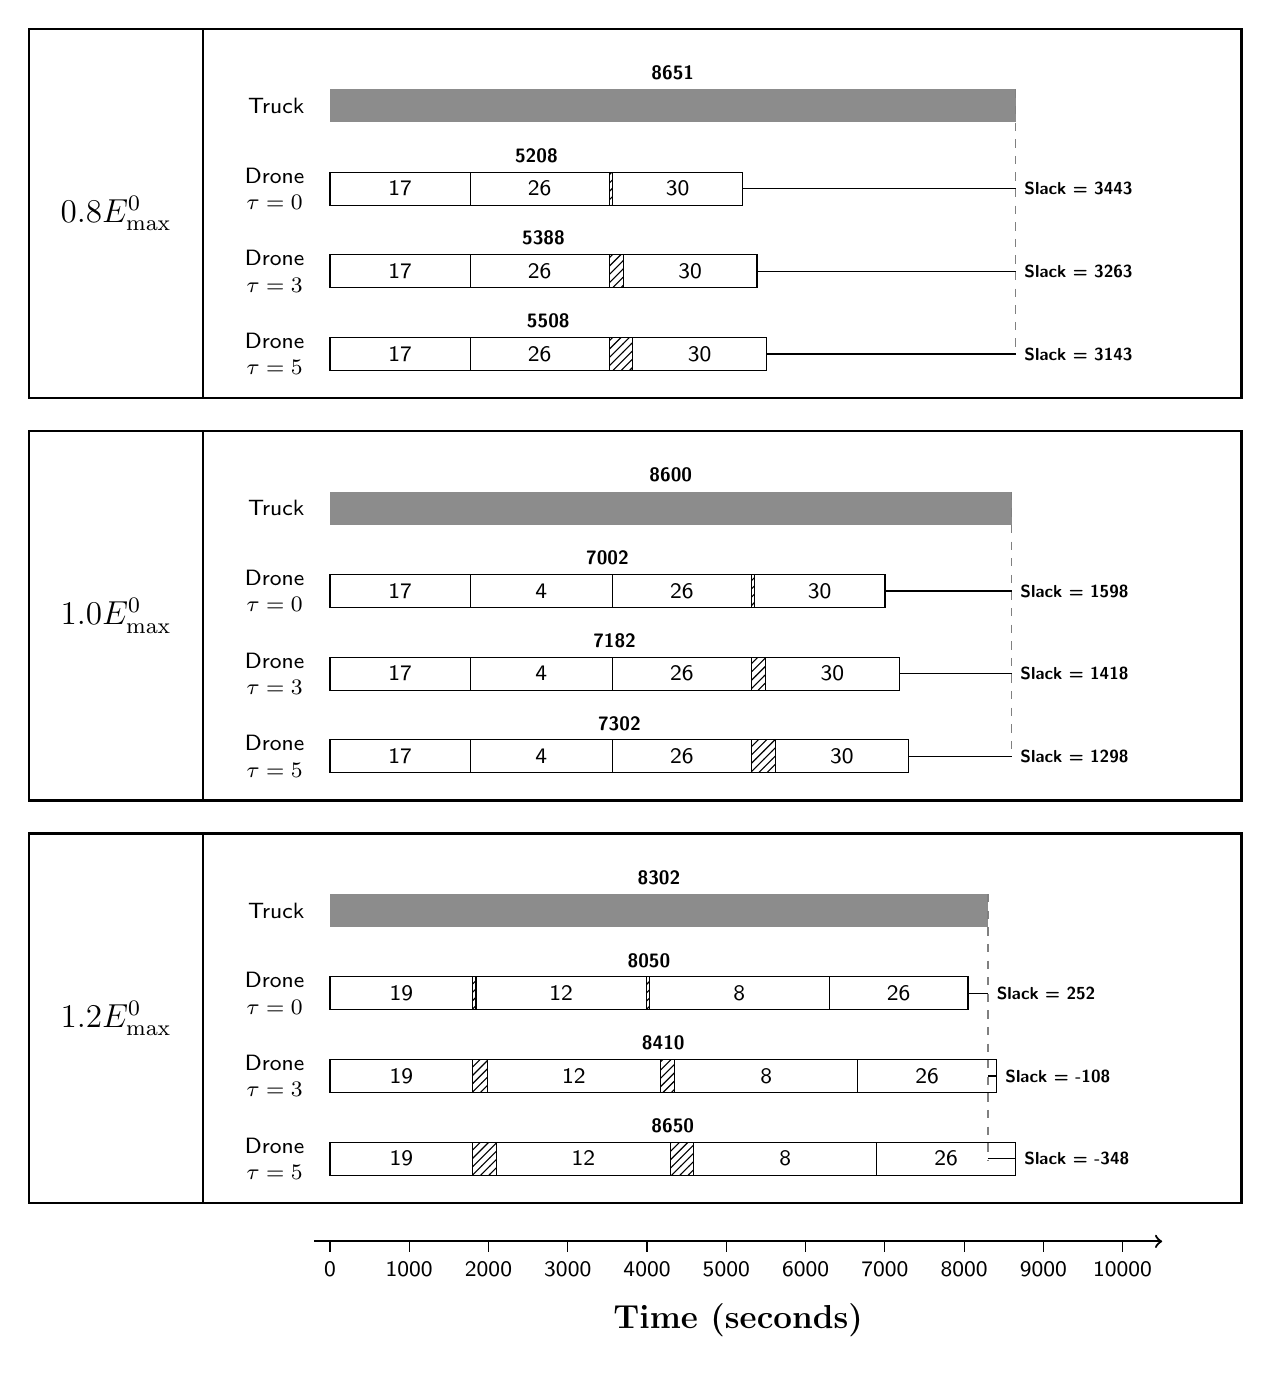
\begin{tikzpicture}[x=0.001cm, y=0.7cm, font=\sffamily\footnotesize]

    % ==========================================
    % BLOCK 1: 0.8 E_max
    % ==========================================
    \draw[thick] (-3800, -0.5) rectangle (11500, 6.2);
    \draw[thick] (-1600, -0.5) -- (-1600, 6.2);
    \node at (-2700, 2.85) {\large $0.8E_{\max}^{0}$};

    % 1.1 TRUCK
    \fill[gray!90] (0, 4.5) rectangle (8651, 5.1);
    \node[left] at (-200, 4.8) {Truck};
    \node[above=0pt] at (4325, 5.1) {\scriptsize\textbf{8651}}; 
    \draw[dashed, gray] (8651, 5.1) -- (8651, 0.3);

    % 1.2 DRONE tau = 0
    \node[left, align=center] at (-200, 3.3) {Drone \\ $\tau=0$};
    \draw (0, 3.0) rectangle (1770, 3.6); \node at (885, 3.3) {17};
    \draw (1770, 3.0) rectangle (3522, 3.6); \node at (2646, 3.3) {26};
    \draw[pattern=north east lines] (3522, 3.0) rectangle (3562, 3.6); 
    \draw (3562, 3.0) rectangle (5208, 3.6); \node at (4385, 3.3) {30};
    \node[above=0pt] at (2604, 3.6) {\scriptsize\textbf{5208}};
    \draw (5208, 3.3) -- (8651, 3.3); 
    \node[right, scale=0.9] at (8651, 3.3) {\scriptsize\textbf{Slack = 3443}};

    % 1.3 DRONE tau = 3
    \node[left, align=center] at (-200, 1.8) {Drone \\ $\tau=3$};
    \draw (0, 1.5) rectangle (1770, 2.1); \node at (885, 1.8) {17};
    \draw (1770, 1.5) rectangle (3522, 2.1); \node at (2646, 1.8) {26};
    \draw[pattern=north east lines] (3522, 1.5) rectangle (3702, 2.1); 
    \draw (3702, 1.5) rectangle (5388, 2.1); \node at (4545, 1.8) {30};
    \node[above=0pt] at (2694, 2.1) {\scriptsize\textbf{5388}};
    \draw (5388, 1.8) -- (8651, 1.8); 
    \node[right, scale=0.9] at (8651, 1.8) {\scriptsize\textbf{Slack = 3263}};

    % 1.4 DRONE tau = 5
    \node[left, align=center] at (-200, 0.3) {Drone \\ $\tau=5$};
    \draw (0, 0.0) rectangle (1770, 0.6); \node at (885, 0.3) {17};
    \draw (1770, 0.0) rectangle (3522, 0.6); \node at (2646, 0.3) {26};
    \draw[pattern=north east lines] (3522, 0.0) rectangle (3822, 0.6); 
    \draw (3822, 0.0) rectangle (5508, 0.6); \node at (4665, 0.3) {30};
    \node[above=0pt] at (2754, 0.6) {\scriptsize\textbf{5508}};
    \draw (5508, 0.3) -- (8651, 0.3); 
    \node[right, scale=0.9] at (8651, 0.3) {\scriptsize\textbf{Slack = 3143}};


    % ==========================================
    % BLOCK 2: 1.0 E_max
    % ==========================================
    \draw[thick] (-3800, -7.8) rectangle (11500, -1.1);
    \draw[thick] (-1600, -7.8) -- (-1600, -1.1);
    \node at (-2700, -4.45) {\large $1.0E_{\max}^{0}$};

    % 2.1 TRUCK
    \fill[gray!90] (0, -2.8) rectangle (8600, -2.2);
    \node[left] at (-200, -2.5) {Truck};
    \node[above=0pt] at (4300, -2.2) {\scriptsize\textbf{8600}};
    \draw[dashed, gray] (8600, -2.2) -- (8600, -7.0);

    % 2.2 DRONE tau = 0
    \node[left, align=center] at (-200, -4.0) {Drone \\ $\tau=0$};
    \draw (0, -4.3) rectangle (1770, -3.7); \node at (885, -4.0) {17};
    \draw (1770, -4.3) rectangle (3564, -3.7); \node at (2667, -4.0) {4};
    \draw (3564, -4.3) rectangle (5316, -3.7); \node at (4440, -4.0) {26};
    \draw[pattern=north east lines] (5316, -4.3) rectangle (5356, -3.7); 
    \draw (5356, -4.3) rectangle (7002, -3.7); \node at (6179, -4.0) {30};
    \node[above=0pt] at (3501, -3.7) {\scriptsize\textbf{7002}};
    \draw (7002, -4.0) -- (8600, -4.0); 
    \node[right, scale=0.9] at (8600, -4.0) {\scriptsize\textbf{Slack = 1598}};

    % 2.3 DRONE tau = 3
    \node[left, align=center] at (-200, -5.5) {Drone \\ $\tau=3$};
    \draw (0, -5.8) rectangle (1770, -5.2); \node at (885, -5.5) {17};
    \draw (1770, -5.8) rectangle (3564, -5.2); \node at (2667, -5.5) {4};
    \draw (3564, -5.8) rectangle (5316, -5.2); \node at (4440, -5.5) {26};
    \draw[pattern=north east lines] (5316, -5.8) rectangle (5496, -5.2); 
    \draw (5496, -5.8) rectangle (7182, -5.2); \node at (6339, -5.5) {30};
    \node[above=0pt] at (3591, -5.2) {\scriptsize\textbf{7182}};
    \draw (7182, -5.5) -- (8600, -5.5); 
    \node[right, scale=0.9] at (8600, -5.5) {\scriptsize\textbf{Slack = 1418}};

    % 2.4 DRONE tau = 5
    \node[left, align=center] at (-200, -7.0) {Drone \\ $\tau=5$};
    \draw (0, -7.3) rectangle (1770, -6.7); \node at (885, -7.0) {17};
    \draw (1770, -7.3) rectangle (3564, -6.7); \node at (2667, -7.0) {4};
    \draw (3564, -7.3) rectangle (5316, -6.7); \node at (4440, -7.0) {26};
    \draw[pattern=north east lines] (5316, -7.3) rectangle (5616, -6.7); 
    \draw (5616, -7.3) rectangle (7302, -6.7); \node at (6459, -7.0) {30};
    \node[above=0pt] at (3651, -6.7) {\scriptsize\textbf{7302}};
    \draw (7302, -7.0) -- (8600, -7.0); 
    \node[right, scale=0.9] at (8600, -7.0) {\scriptsize\textbf{Slack = 1298}};


    % ==========================================
    % BLOCK 3: 1.2 E_max
    % ==========================================
    \draw[thick] (-3800, -15.1) rectangle (11500, -8.4);
    \draw[thick] (-1600, -15.1) -- (-1600, -8.4);
    \node at (-2700, -11.75) {\large $1.2E_{\max}^{0}$};

    % 3.1 TRUCK
    \fill[gray!90] (0, -10.1) rectangle (8302, -9.5);
    \node[left] at (-200, -9.8) {Truck};
    \node[above=0pt] at (4151, -9.5) {\scriptsize\textbf{8302}};
    \draw[dashed, gray] (8302, -9.5) -- (8302, -14.35);

    % 3.2 DRONE tau = 0
    \node[left, align=center] at (-200, -11.3) {Drone \\ $\tau=0$};
    \draw (0, -11.6) rectangle (1802, -11.0); \node at (901, -11.3) {19};
    \draw[pattern=north east lines] (1802, -11.6) rectangle (1842, -11.0); 
    \draw (1842, -11.6) rectangle (3992, -11.0); \node at (2917, -11.3) {12};
    \draw[pattern=north east lines] (3992, -11.6) rectangle (4032, -11.0); 
    \draw (4032, -11.6) rectangle (6298, -11.0); \node at (5165, -11.3) {8};
    \draw (6298, -11.6) rectangle (8050, -11.0); \node at (7174, -11.3) {26};
    \node[above=0pt] at (4025, -11.0) {\scriptsize\textbf{8050}};
    \draw (8050, -11.3) -- (8302, -11.3); 
    \node[right, scale=0.9] at (8302, -11.3) {\scriptsize\textbf{Slack = 252}};

    % 3.3 DRONE tau = 3
    \node[left, align=center] at (-200, -12.8) {Drone \\ $\tau=3$};
    \draw (0, -13.1) rectangle (1802, -12.5); \node at (901, -12.8) {19};
    \draw[pattern=north east lines] (1802, -13.1) rectangle (1982, -12.5); 
    \draw (1982, -13.1) rectangle (4172, -12.5); \node at (3077, -12.8) {12};
    \draw[pattern=north east lines] (4172, -13.1) rectangle (4352, -12.5); 
    \draw (4352, -13.1) rectangle (6658, -12.5); \node at (5505, -12.8) {8};
    \draw (6658, -13.1) rectangle (8410, -12.5); \node at (7534, -12.8) {26};
    \node[above=0pt] at (4205, -12.5) {\scriptsize\textbf{8410}};
    \draw (8302, -12.8) -- (8410, -12.8); 
    \node[right, scale=0.9] at (8410, -12.8) {\scriptsize\textbf{Slack = -108}}; 

    % 3.4 DRONE tau = 5
    \node[left, align=center] at (-200, -14.3) {Drone \\ $\tau=5$};
    \draw (0, -14.6) rectangle (1802, -14.0); \node at (901, -14.3) {19};
    \draw[pattern=north east lines] (1802, -14.6) rectangle (2102, -14.0); 
    \draw (2102, -14.6) rectangle (4292, -14.0); \node at (3197, -14.3) {12};
    \draw[pattern=north east lines] (4292, -14.6) rectangle (4592, -14.0); 
    \draw (4592, -14.6) rectangle (6898, -14.0); \node at (5745, -14.3) {8};
    \draw (6898, -14.6) rectangle (8650, -14.0); \node at (7774, -14.3) {26};
    \node[above=0pt] at (4325, -14.0) {\scriptsize\textbf{8650}};
    \draw (8302, -14.3) -- (8650, -14.3); 
    \node[right, scale=0.9] at (8650, -14.3) {\scriptsize\textbf{Slack = -348}}; 


    % ==========================================
    % TRỤC THỜI GIAN (X-AXIS)
    % ==========================================
    \draw[->, thick] (-200, -15.8) -- (10500, -15.8);

    \foreach \x in {0,1000,2000,3000,4000,5000,6000,7000,8000,9000,10000} {
        \draw (\x, -15.8) -- (\x, -16.0);
        \node[below] at (\x, -16.0) {\x};
    }

    
    \node[below, font=\bfseries\large] at (5150, -16.75) {Time (seconds)};

    \end{tikzpicture}
    }
    \caption{Illustration of slack reduction under increasing energy capacity ($E_{\max}$) for instance 30--c--0--e.}
    
    \captionsetup{justification=raggedright,singlelinecheck=false}
    \caption*{%
    \hspace{0.1\textwidth}%
    \footnotesize
    \textbf{Note:}\;
    
\begin{tikzpicture}[baseline=-0.08ex]
        \draw[pattern=north east lines] (0,0) rectangle (0.18,0.30);
    \end{tikzpicture}
    \hspace{0.2em}denotes battery swap time.
    }
    \captionsetup{justification=centering,singlelinecheck=true}
    
    \label{fig:slack_ex}
\end{figure}

The slack values at the baseline configuration ($\tau_{\mathrm{swap}} = 0$) are 3443s, 1598s, and 252s at $0.8E_{max}$, $1.0E_{max}$, and $1.2E_{max}$, respectively. This shows that, as energy resources increase, the slack reduces dramatically. Specifically, at low-resource configurations ($0.8E_{max}$ and $1.0E_{max}$), this slack is substantial and effectively absorbs swap-time delays. However, as energy resources increase to $1.2E_{max}$, the slack diminishes to only 252s. In this high-resource configuration, the drone's schedule becomes tightly coupled with the makespan. Therefore, it is critical to explicitly account for swap-time. Otherwise, the drone's completion time may exceed the truck's operational horizon, causing the drone to become the bottleneck and significantly increasing makespan deviation.

Although the deviation within drone-bottleneck runs decreases in both models as resource levels increase, due to the improved operational flexibility of drones, this effect is dominated by the combination of smaller slack and a higher probability of drone-bottleneck runs, resulting in a larger overall deviation.


\section{Conclusions}
\label{sec:conclusions}

This paper investigates the impact of battery swap-time in the Parallel Drone Scheduling Traveling Salesman Problem (PDSTSP).
We develop two problem variants --- a time-based model and an energy-based model --- and for each, we compare two ways of handling swap-time: ignoring it during optimization and only accounting for it afterward through re-evaluation, versus integrating it explicitly within the optimization process itself.

To solve the resulting problems, we employ three complementary approaches:
a mixed-integer linear programming (MILP) formulation,
a branch-cut-and-price (BCP) model using VRPSolver,
and a hybrid genetic search (HGS) algorithm.
The exact methods provide optimal or near-optimal benchmarks for smaller problem limits,
while the HGS efficiently scales to larger problem sizes up to 100 nodes and enables extensive sensitivity analysis.

Across all computational experiments, we observe that ignoring swap-time during optimization leads to systematic underestimation of the makespan when solutions are re-evaluated under realistic swapping operations.
In contrast, explicitly integrating swap-time produces solutions that remain stable and consistent.
This pattern holds for both time-based and energy-based formulations; crucially, our sensitivity analysis reveals that increasing drone resource capacities actually worsens this underestimation, rather than mitigating it.

The results provide a clear answer to the central question of this study:
battery swap-time should be explicitly integrated into PDSTSP models.
Moreover, as drone delivery systems move toward real-world deployment, accounting for battery swap-time will be essential to closing the gap between theoretical schedules and achievable performance.

Future research may extend this framework to other truck–drone routing variants, including synchronized launch–recovery models, multiple-truck systems, time-window constraints, and stochastic travel or energy conditions.

\bibliographystyle{apalike}
\bibliography{pdstsp,pdstsp_vrpsolver_additions}
\end{document}